%\clearpage
\fancyhead[LO,RE]{ANEXOS}
\appendix
\renewcommand{\appendixname}{Anexos}
\renewcommand{\appendixtocname}{Anexos}
\renewcommand{\appendixpagename}{Anexos}
\clearpage
\addappheadtotoc
%\appendixpage %Agrega una pagina en blanco q en el medio Dice Anexo en grande..


\chapter{Comparación de plataformas de hardware}
        \begin{longtable}{|p{4cm}|p{5cm}|p{5cm}|}
            \hline
            \multicolumn{3}{| c |}{\textbf{Comparación de plataformas de hardware}}\\
            \hline
            Criterio de Comparación & Arduino\textsuperscript{\textregistered} & Raspberry\textsuperscript{\textregistered} pi\\
            \hline
            \endfirsthead
             
            \hline
            \multicolumn{3}{|c|}{Continuación de la tabla \ref{CompHard}}\\
            \hline
            Criterio de Comparación & Arduino\textsuperscript{\textregistered} & Raspberry\textsuperscript{\textregistered} pi\\
            \hline
            \endhead
             
            \hline
            \endfoot
             
            \hline
            %\multicolumn{3}{| c |}{End of Table}\\
            %\hline
            \caption{Comparación entre Arduino y Raspberry Pi \label{CompHard}}\\
            \endlastfoot
            
            Precio & \$440 (USD 17,00) & \$1900 (USD 61,00)
            \\ \hline
            Manejo de sensores & Digitales y analógicos & Digitales y analógicos
            \\ \hline
            Capacidad de procesamiento, memoria y almacenamiento & Procesador de 8 bits a 16Mhz, memoria de 2KB, sin almacenamiento (sin slot de expansión). & Procesador de 64 bits a 1.4Ghz, memoria de 1GB, sin almacenamiento (Slot memoria SD).
            \\ \hline
            Conectividad & Conexión USB (tipo B) x 1. Pueden adicionarse Shields Ethernet, Bluetooth o WiFi. & Conexión USB (tipo A) x 4, Ethernet 100M, WiFi 802.11n/ac, Bluetooth.
            \\ \hline
            Tamaño & 7.6 x 1.9 x 6.4 cm. & 8.6cm x 5.4cm x 1.7cm.
            \\ \hline

            Lenguaje de programación & Lenguaje Bajo Nivel. Gran comunidad y soporte. Se requiere de un computador para el desarrollo. & Lenguaje Alto Nivel. Gran comunidad y soporte. Se desarrolla directamente en el dispositivo.
            \\ \hline
                
            Persistencia de datos ante pérdida de alimentación eléctrica & Ninguna & Al utilizar una memoria SD, se obtiene persistencia de datos.
            \\ \hline

            \end{longtable}

%---------------------------------------------------------------------------------
    \begin{minipage}{0.95\textwidth}
\chapter{Diagrama de base de datos del componente de hardware}
        \centering
        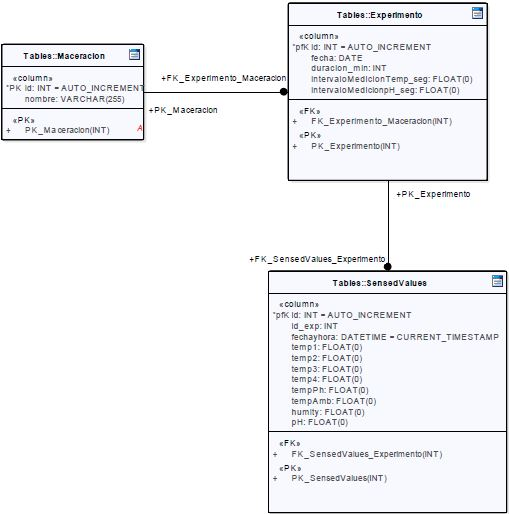
\includegraphics[scale=0.65]{diagramaBD-Rasp.jpg}
        \captionof{figure}{Diagrama de diseño de Base de Datos}
        \label{fig:DiagramaBdRasp}
    
    \end{minipage}
    
%------------------ INTERFAZ ----------------
\chapter{Comparación de tecnologías inalámbricas para interfaz Hardware - Software}

\begin{table}[h]
    \centering
    
    \begin{tabularx}{\textwidth}{|X|X|X|}
        \hline
        \multicolumn{3}{|c|}{\textbf{Comparación de tecnologías inalámbricas}}
        \\
        \hline
            
        & Bluetooth\textsuperscript{\textregistered} & Wi-Fi\textsuperscript{\textregistered}  \\ \hline \hline
             
        Frecuencia & 2.4 GHz & 2.4, 3.6, 5 GHz \\ \hline 
                     
        Ancho de banda (Bandwidth) & Bajo (800 kbps) & Alto (11 Mbps en 802.11b) \\ \hline
                     
        Autoridad de especificación & Bluetooth SIG\footnote{ Bluetooth Special Interest Group, asociación privada sin ánimo de lucro} & IEEE, WECA \\ \hline
                     
        Seguridad & Poco seguro & Más seguro \\ \hline
                     
        Dispositivos principales & Teléfonos inteligentes, ratones, teclados, etc & Notebook, Computadoras de escritorio, Servidores, TV, Teléfonos inteligentes, etc\\ \hline
                     
        Requerimientos de Hardware & Adaptador Bluetooth en todos los dispositivos & Adaptadores inalámbricos (Wireless) en todos los dispositivos de la red, wireless router y/o wireless access point \\ \hline
                    
        Cantidad de dispositivos conectados & Solo dos & Múltiples\\ \hline
                     
        Rango & 5-30 metros & 32-300 metros \\ \hline
                     
        Consumo de Energía & Bajo & Alto \\ \hline
                     
        Latencia & 200 ms & 150 ms \\ \hline
                     
        Tasa de transferencia (Bit-rate) & 2.1 Mbps & 600 Mbps\\ \hline
            
    \end{tabularx}
    
    \caption{Comparación de tecnologías inalámbricas Bluetooth\textsuperscript{\textregistered} y Wi-Fi\textsuperscript{\textregistered}}
    \label{tab:ComparacionInterfaz}
\end{table}

%---------------------- MOCK UP ----------------------------------------
 \chapter{Comparativa tecnologías de software para teléfonos móviles}
 \begin{table}[h!]
            \centering
            \begin{tabularx}{\textwidth}{|X|X|X|}
                 \hline
                 \multicolumn{3}{|c|}{Tabla comparativa de tecnologías de software para teléfonos móviles}\\
                 \hline
                 Criterios de comparación & Android & iOS \\
                 \hline
                 \hline
                 
                 Porcentaje Mercado (Arg) & 75\% & 19\%  \\
                 \hline
                 
                 Porcentaje Mercado Internacional & 85\% & 14,7\% \\
                 \hline
                 
                 Comunidad de desarrolladores & Muy grande & Amplia pero acorde al número de usuarios\\
                 \hline
                 
                  Entornos desarrollo Propia & Android Studio & Xcode\\
                 \hline
                 
                 Lenguaje de desarrollo & Java, C, C++ y Kotlin & Swift, C, C++ y objective-C\\
                 \hline
                 
                 Familia del SO & Linux & Unix - BSD\\
                 \hline
                 
                 Complejidad de desarrollo & Alta variedad de dispositivos y versiones del SO & Baja variedad de dispositivos, versiones de SO comunes a la mayoría\\
                 \hline
                 
                 Entorno & Open Source & Entorno cerrado \\
                 \hline
                 
                 Requerimientos para publicación de aplicación & Ninguna & Debe cumplir requisitos de Apple\\
                 \hline
                 
            \end{tabularx}
            \caption{Comparación de plataformas móviles}
            \label{tab:ComparacionPlataformasMoviles}
        \end{table}
    \hfill \break
    \hfill \break
    \hfill \break
    \hfill \break
    \hfill \break
    \hfill \break
    \hfill \break
    \hfill \break
    \hfill \break
        

    \begin{minipage}{0.95\textwidth}
    \chapter{Diseño de interfaz de usuario}
    %\section{Diseño de Interfaz de Usuario}
        \centering
        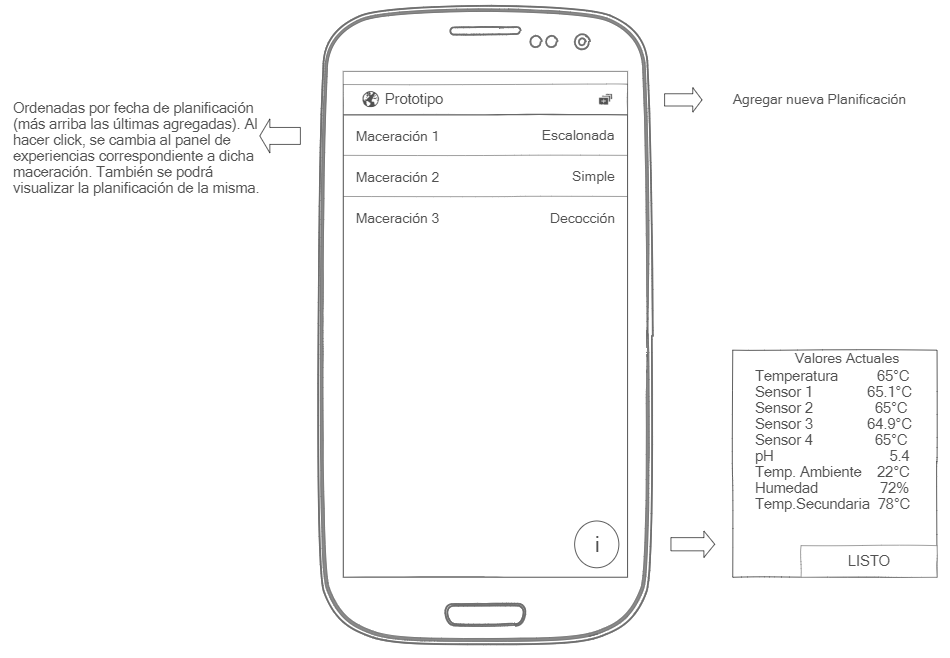
\includegraphics[scale=0.55]{Anexo/MockUp/MainActivity.jpg}
        \captionof{figure}{Pantalla Principal}
        \label{fig:MockUpMainActivity}
    \end{minipage}
    
    \begin{minipage}{0.95\textwidth}

        \centering
        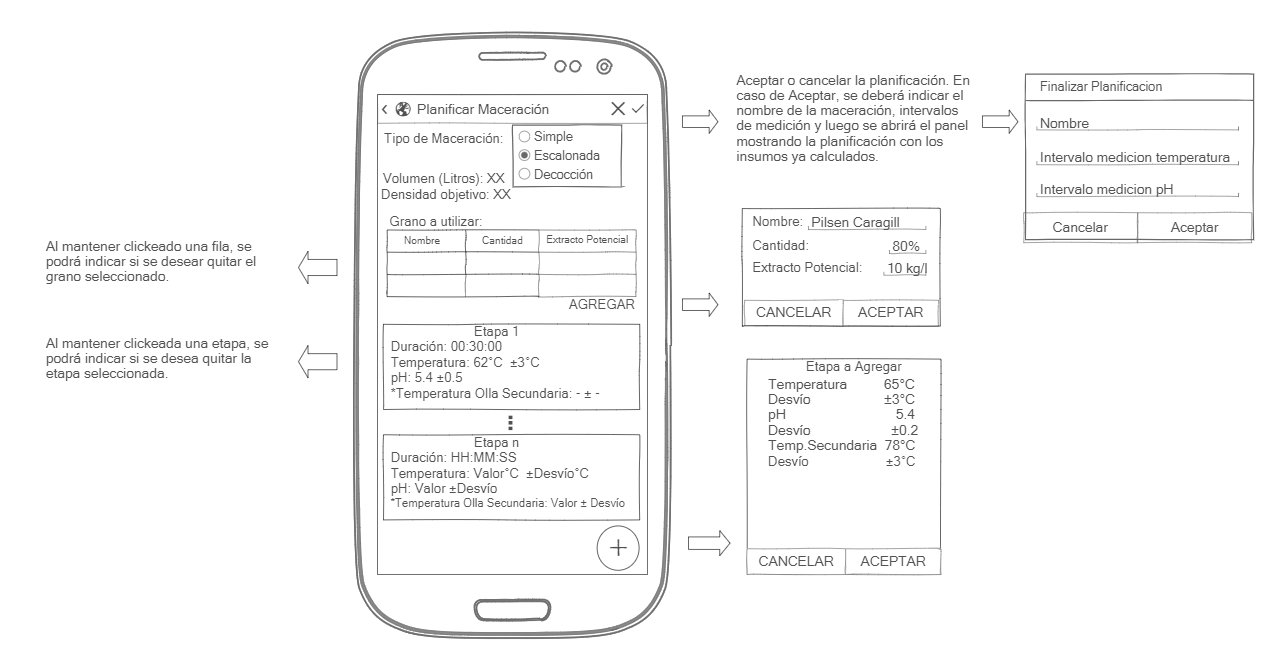
\includegraphics[scale=0.55, angle =90]{Anexo/MockUp/PlanningActivity.jpg}
        \captionof{figure}{Pantalla de planificación de maceración}
        \label{fig:MockUpPlanningActivity}
    \end{minipage}
    
    \begin{minipage}{0.95\textwidth}

        \centering
        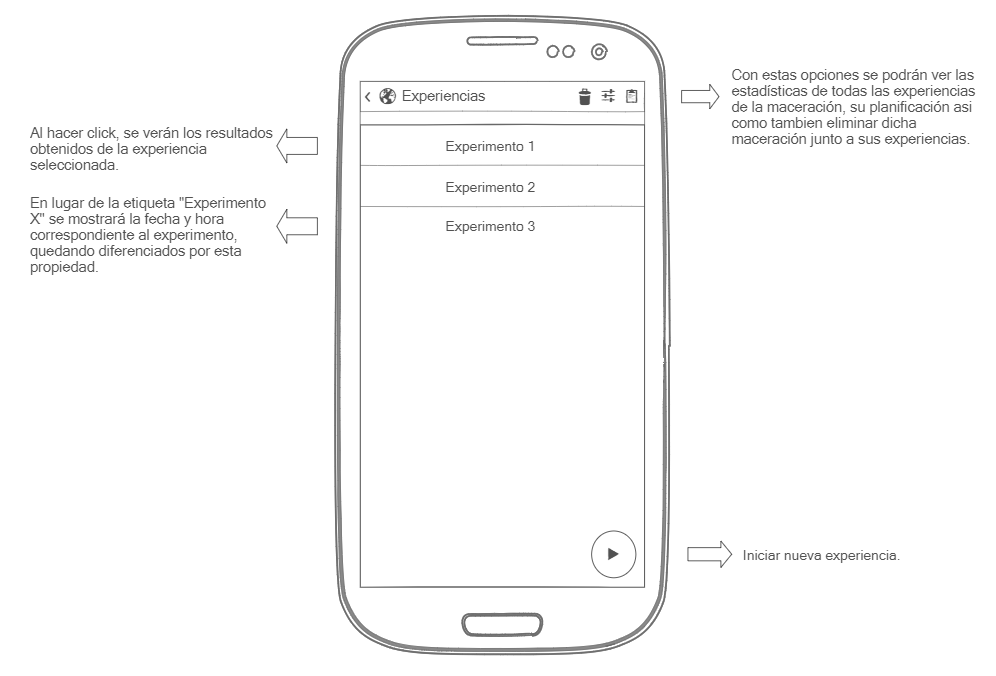
\includegraphics[scale=0.55]{Anexo/MockUp/ExperimentActivity.jpg}
        \captionof{figure}{Pantalla con lista de experimentos de una maceración}
        \label{fig:MockUpExperimentActivity}
    \end{minipage}
    
    \begin{minipage}{0.95\textwidth}

        \centering
        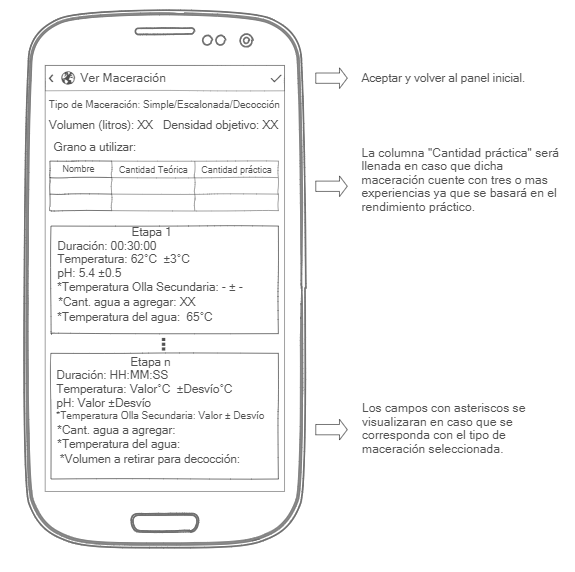
\includegraphics[scale=0.7]{Anexo/MockUp/InfoMash.jpg}
        \captionof{figure}{Pantalla con información de la maceración}
        \label{fig:MockUpInfoMash}
    \end{minipage}
    
    \begin{minipage}{0.95\textwidth}

        \centering
        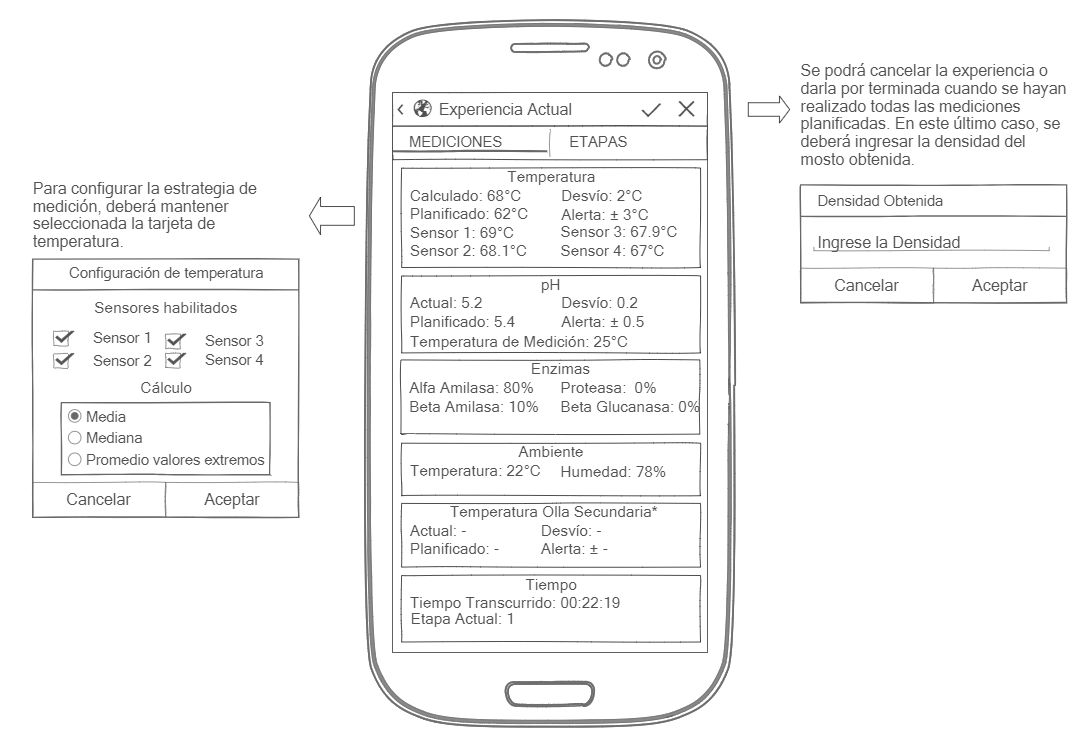
\includegraphics[scale=0.5]{Anexo/MockUp/CurrentExperience-MeasureFragment.jpg}
        \captionof{figure}{Pantalla de mediciones del experimento en ejecución}
        \label{fig:MockUpCurrentExperienceFragment}
    \end{minipage}
    
    \begin{minipage}{0.95\textwidth}

        \centering
        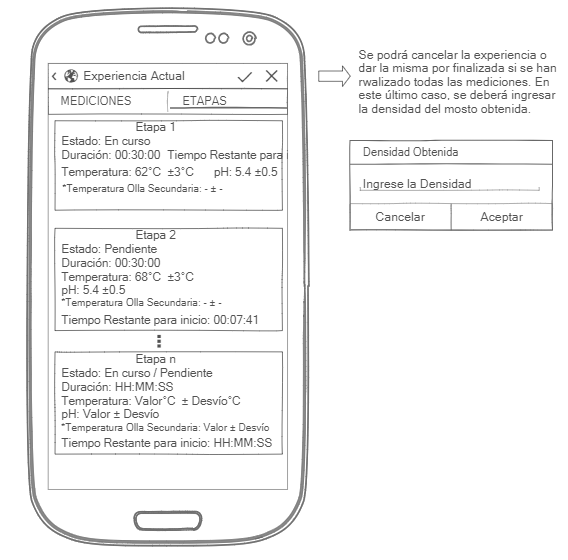
\includegraphics[scale=0.7]{Anexo/MockUp/CurrentExperience-StageFragment.jpg}
        \captionof{figure}{Pantalla con información de las etapas del experimento en ejecución}
        \label{fig:MockUpStageFragment}
    \end{minipage}
    
    \begin{minipage}{0.95\textwidth}

        \centering
        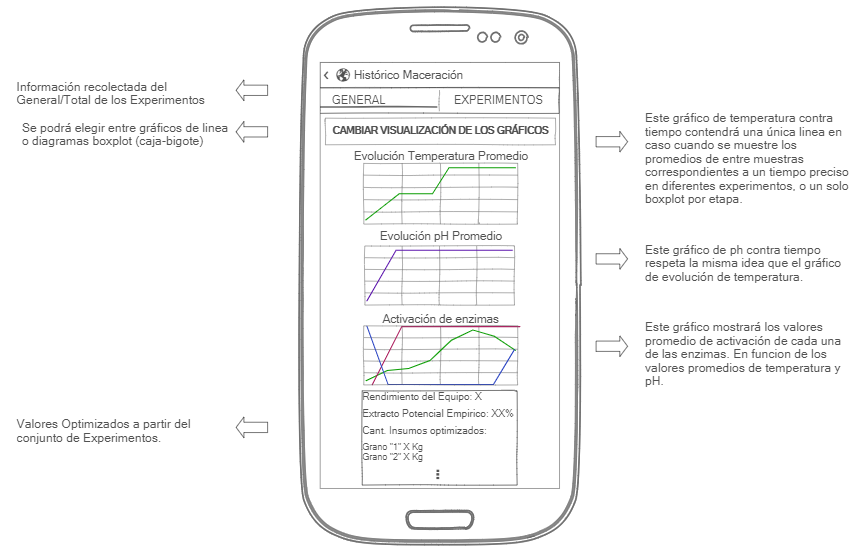
\includegraphics[scale=0.7]{Anexo/MockUp/MashExpHistoryActivity-GeneralFragment.jpg}
        \captionof{figure}{Pantalla con información estadística descriptiva de mediciones y de optimización de insumos y rendimiento}
        \label{fig:MockUpGeneralFragment}
    \end{minipage}
    
    \begin{minipage}{0.95\textwidth}

        \centering
        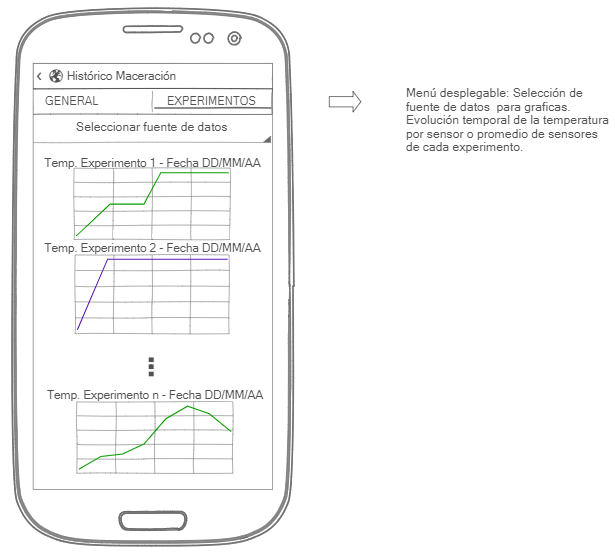
\includegraphics[scale=0.7]{Anexo/MockUp/MashExpHistoryActivity-ExperimentFragment.jpg}
        \captionof{figure}{Pantalla con información estadística descriptiva de mediciones de temperatura de cada experimento}
        \label{fig:MockUpExperimentFragment}
    \end{minipage}
    
   \begin{minipage}{0.95\textwidth}

        \centering
        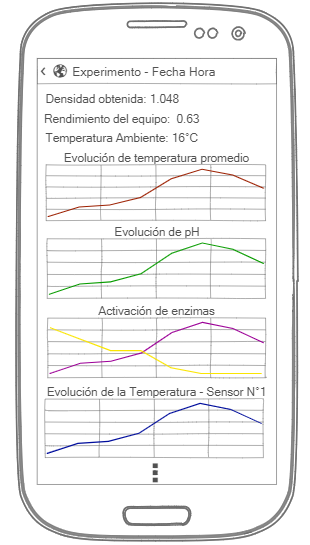
\includegraphics[scale=0.7]{Anexo/MockUp/DetailExperimentActivity.jpg}
        \captionof{figure}{Pantalla con información detalladas de los resultados de cada experimento}
        \label{fig:MockUpDetailExperimentActivity}
    \end{minipage}
    
%-------------------------- DIAGRAMAS DE CLASE --------------------------- 
    \begin{minipage}{0.95\textwidth}
\chapter{Diagramas de clases}
    %\begin{figure}
        \centering
        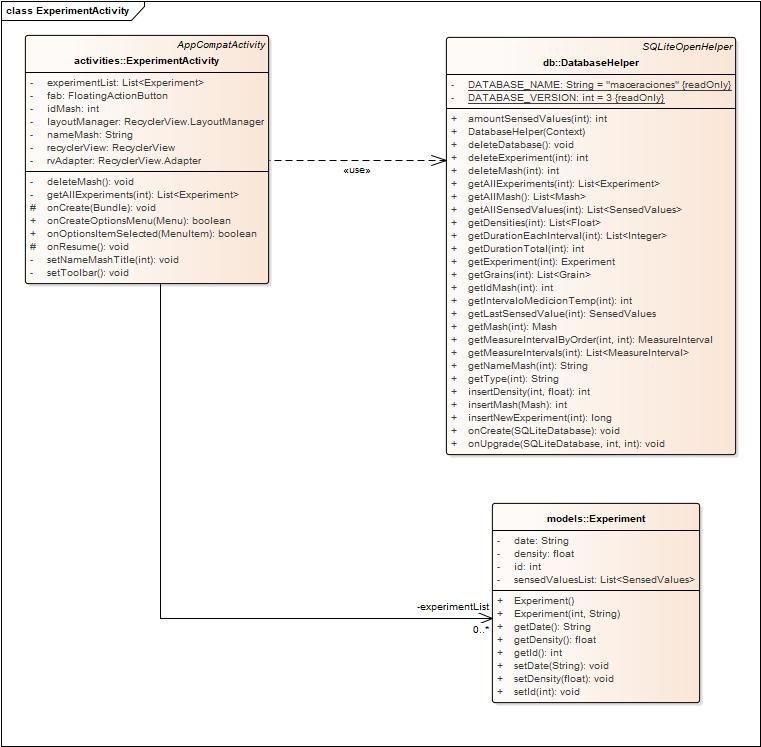
\includegraphics[scale=0.55, angle=90]{Anexo/DiagramasClase/ExperimentActivity.jpg}
        \captionof{figure}{Diagrama de clases de ExperimentActivity}
        \label{fig:DiagClaseExperimentActivity}
    %\end{figure}
    \end{minipage}
    
    %\begin{minipage}{0.95\textwidth}
            \begin{figure}
                \centering
                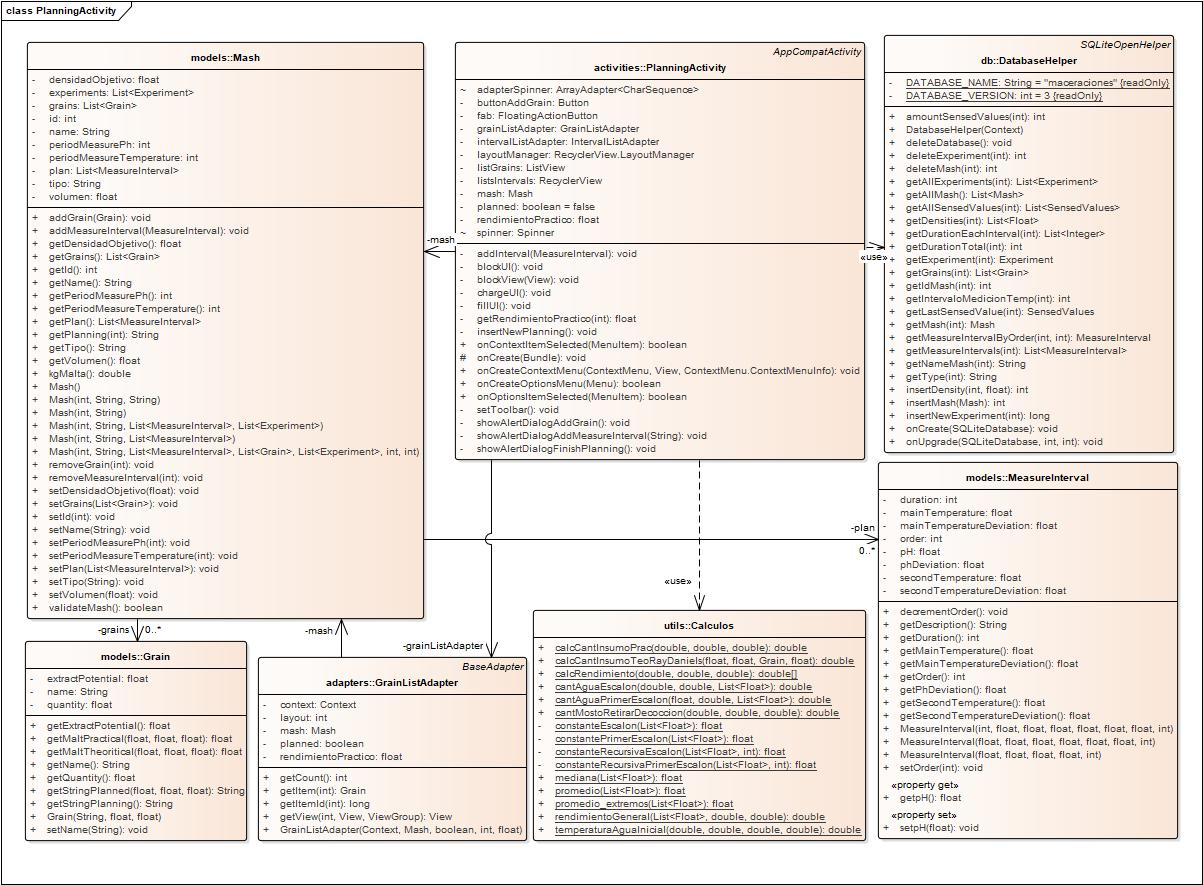
\includegraphics[scale=0.5, angle=90]{Anexo/DiagramasClase/PlanningActivity.jpg}
                \captionof{figure}{Diagrama de clases de PlanningActivity}
                \label{fig:DiagClasePlanningActivity}
            \end{figure}
    %\end{minipage}
    
    
    \begin{figure}
        %\section{Diagramas de clases}
        \centering
        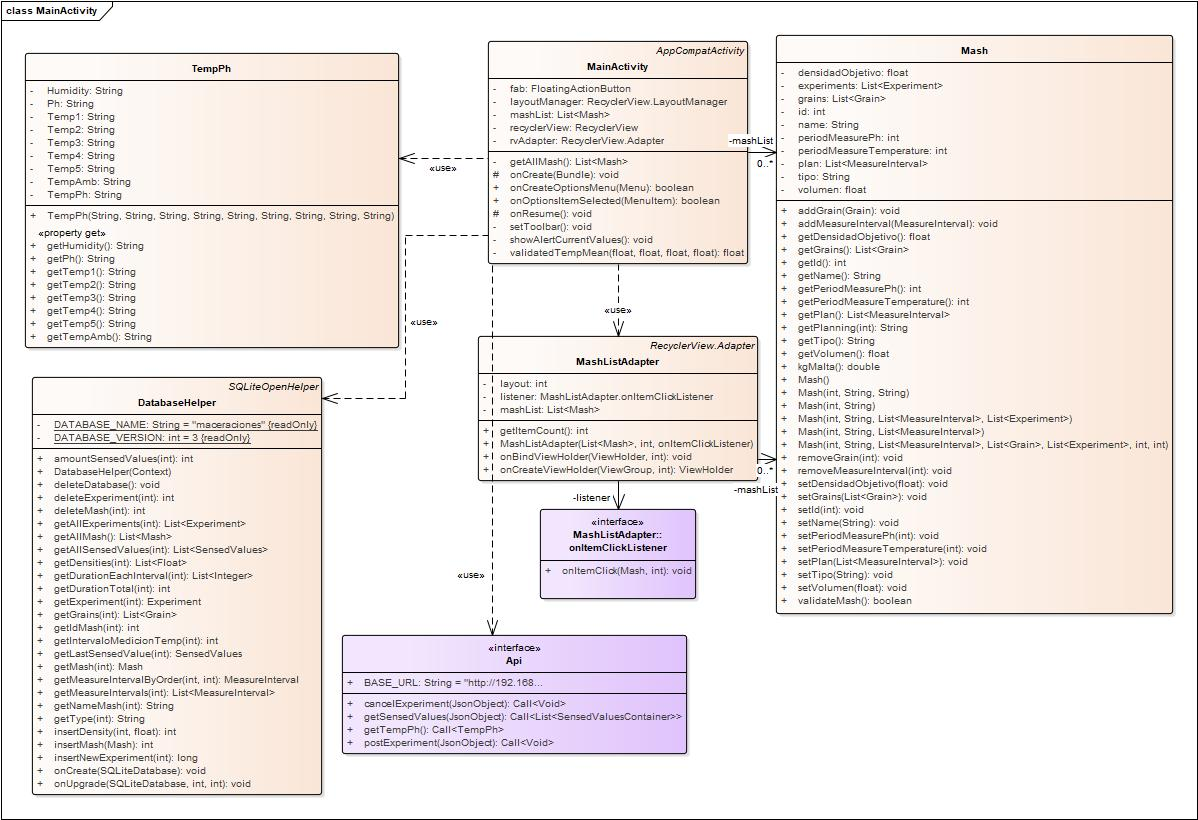
\includegraphics[scale=0.5, angle =90]{Anexo/DiagramasClase/MainActivity.jpg}
        \captionof{figure}{Diagrama de clases de MainActivity}
        \label{fig:DiagClaseMainActivity}
    \end{figure}
    
    
    %\begin{minipage}{0.95\textwidth}
    \begin{figure}
        \centering
        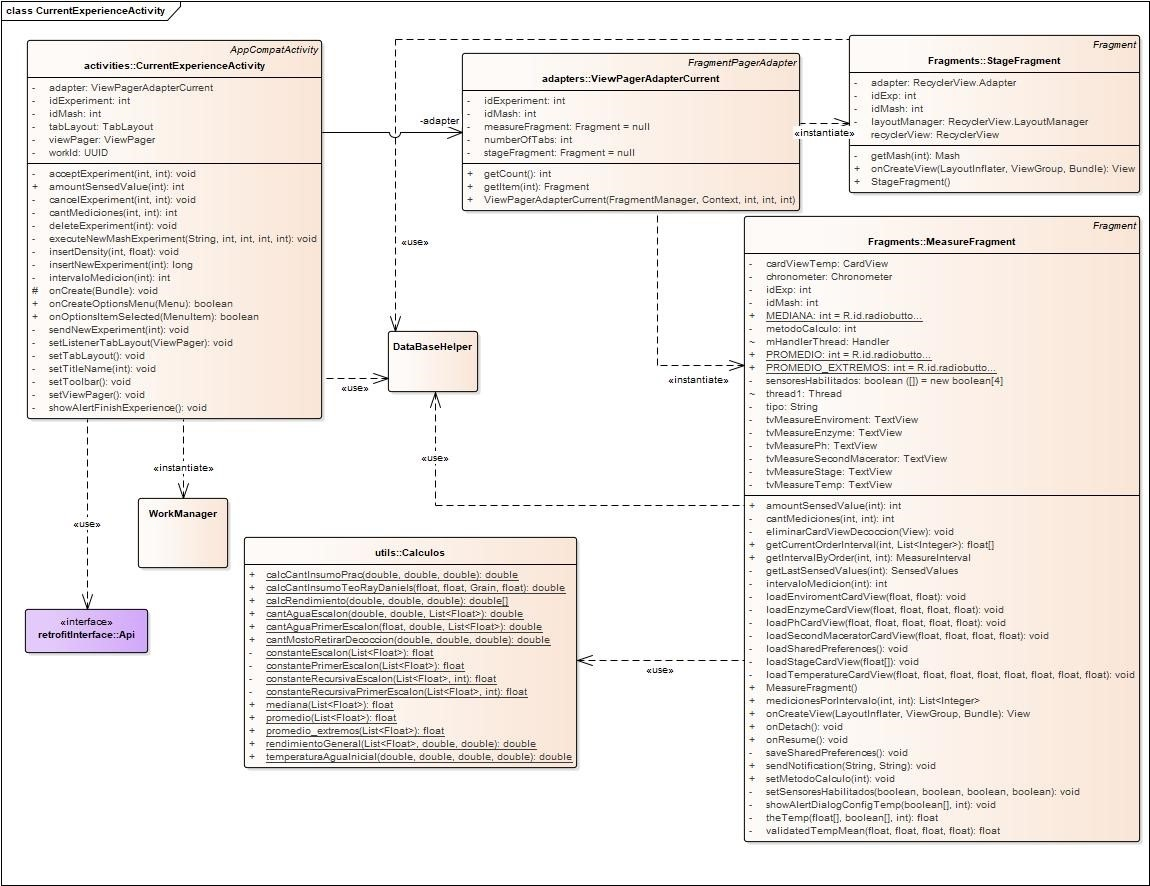
\includegraphics[scale=0.6, angle=90]{Anexo/DiagramasClase/CurrentExperienceActivity-P1.jpg}
        \captionof{figure}{Diagrama de clases de CurrentExperienceActivity - Parte 1}
        \label{fig:DiagClaseCurrentExperienceActivityP1}
    \end{figure}
    %\end{minipage}
    
    %\begin{minipage}{0.95\textwidth}
    \begin{figure}
        \centering
        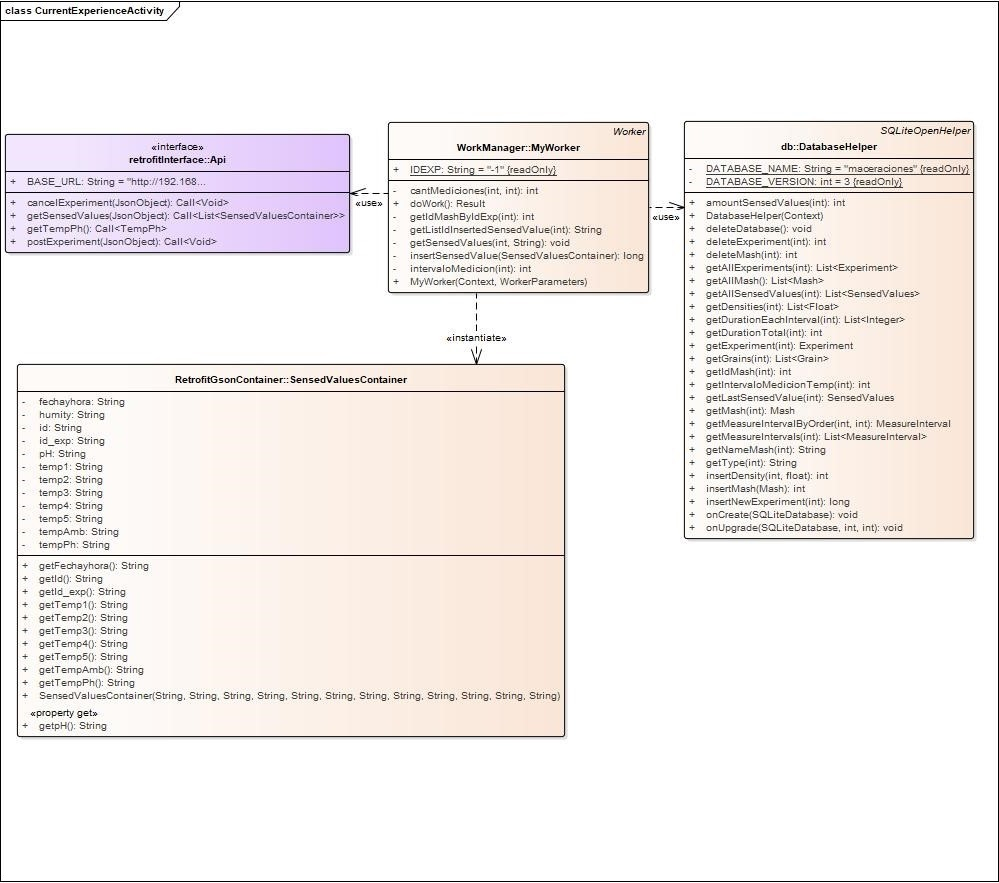
\includegraphics[scale=0.6, angle=90]{Anexo/DiagramasClase/CurrentExperienceActivity-P2.jpg}
        \captionof{figure}{Diagrama de clases de CurrentExperienceActivity - Parte 2}
        \label{fig:DiagClaseCurrentExperienceActivityP2}
    \end{figure}
    %\end{minipage}
    
    %\begin{minipage}{0.95\textwidth}
        \begin{figure}
        \centering
        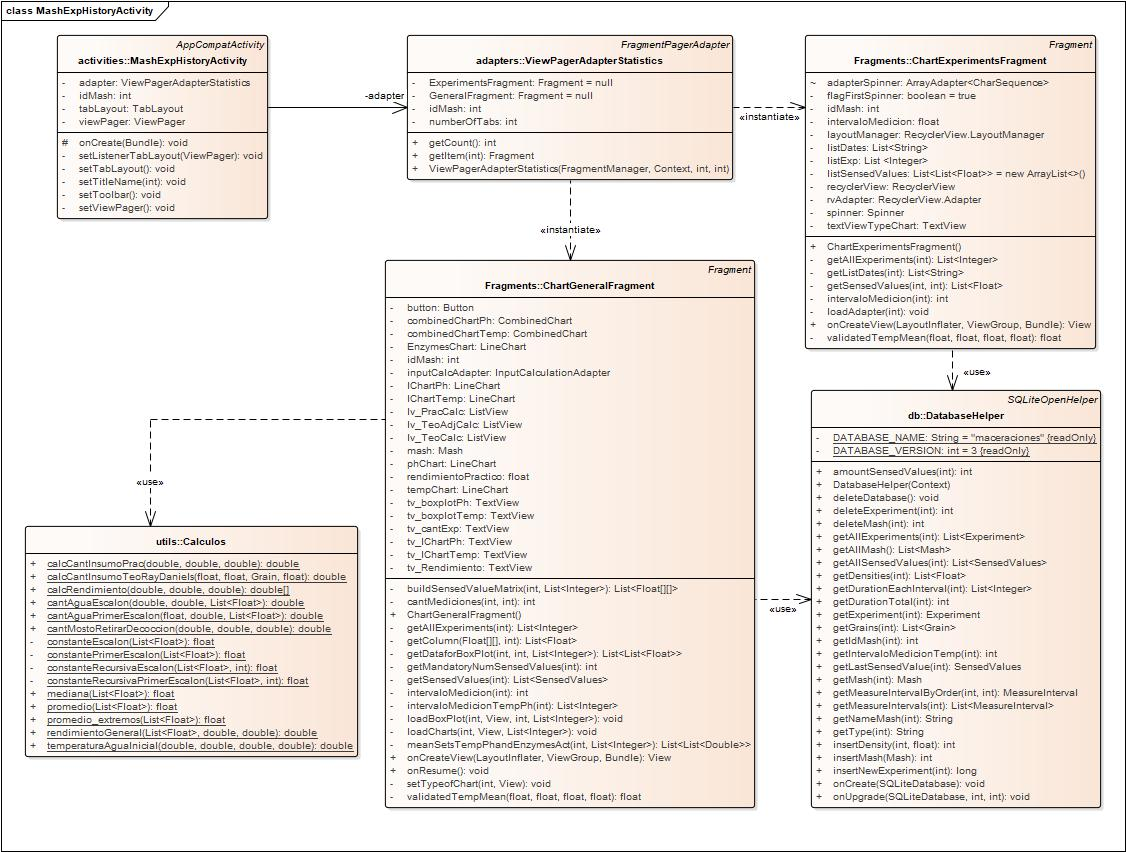
\includegraphics[scale=0.5, angle=90]{Anexo/DiagramasClase/MashExpHistoryActivity.jpg}
        \captionof{figure}{Diagrama de clases de MashExpHistoryActivity}
        \label{fig:DiagClaseMashExpHistoryActivity}
        \end{figure}
    %\end{minipage}
    
    %\begin{minipage}{0.95\textwidth}
        \begin{figure}
        \centering
        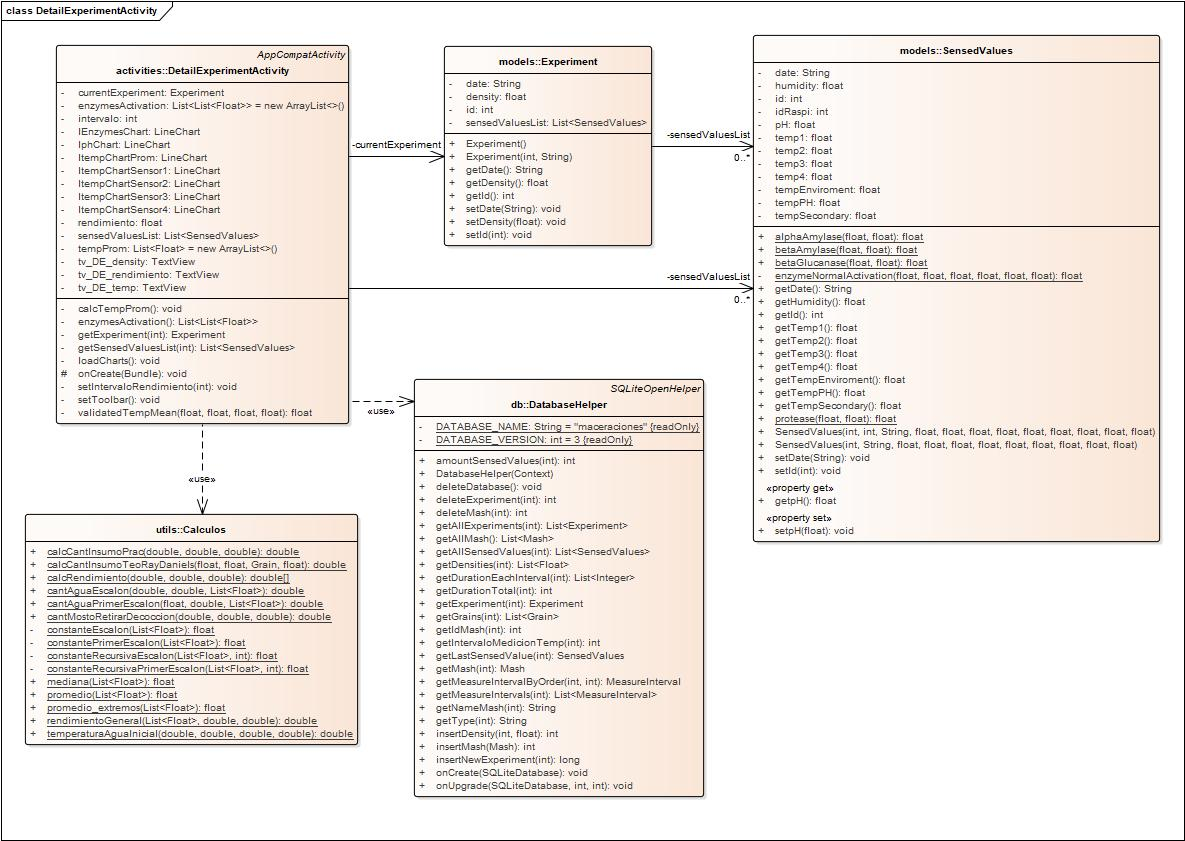
\includegraphics[scale=0.5, angle=90]{Anexo/DiagramasClase/DetailExperimentActivity.jpg}
        \captionof{figure}{Diagrama de clases de DetailExperimentActivity}
        \label{fig:DiagClaseDetailExperimentActivity}
        \end{figure}
    %\end{minipage}
    
    \begin{figure}
        \centering
        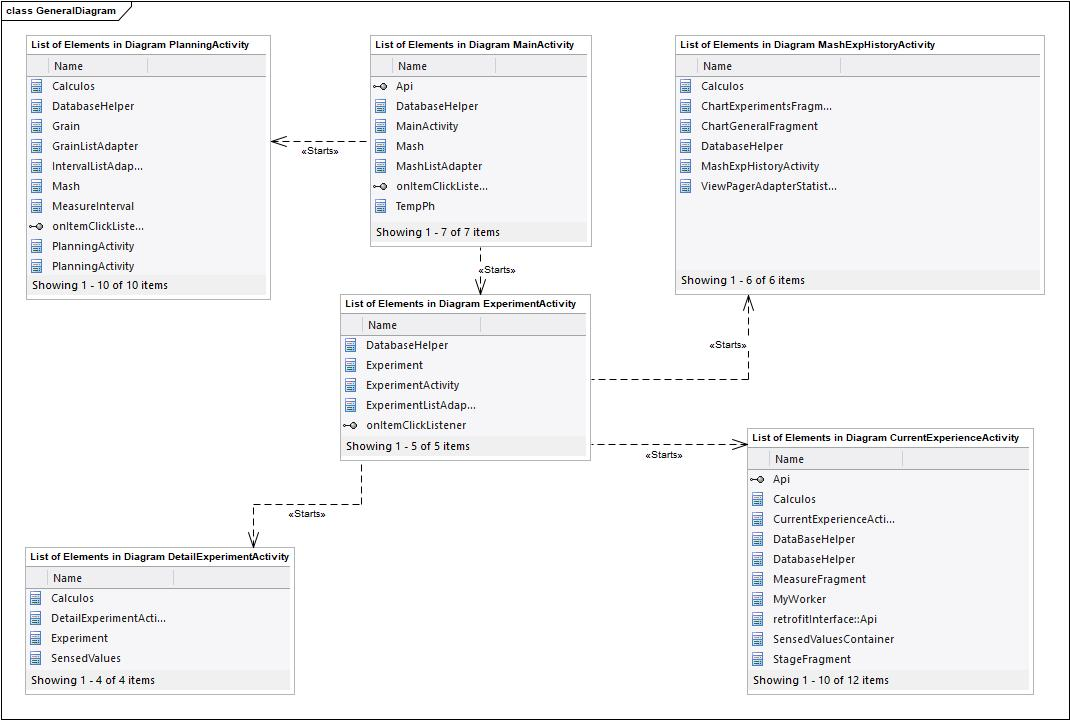
\includegraphics[scale=0.5, angle=90]{Anexo/DiagramasClase/GeneralDiagram.jpg}
        \captionof{figure}{Diagrama General de la Aplicación}
        \label{fig:DiagGeneral}
        \end{figure}
    
    %\begin{minipage}{0.95\textwidth}
    %\begin{minipage}{0.95\textwidth}
\chapter{Fotografías de prueba de campo}
    \label{AnexoFotografias}
        \centering
        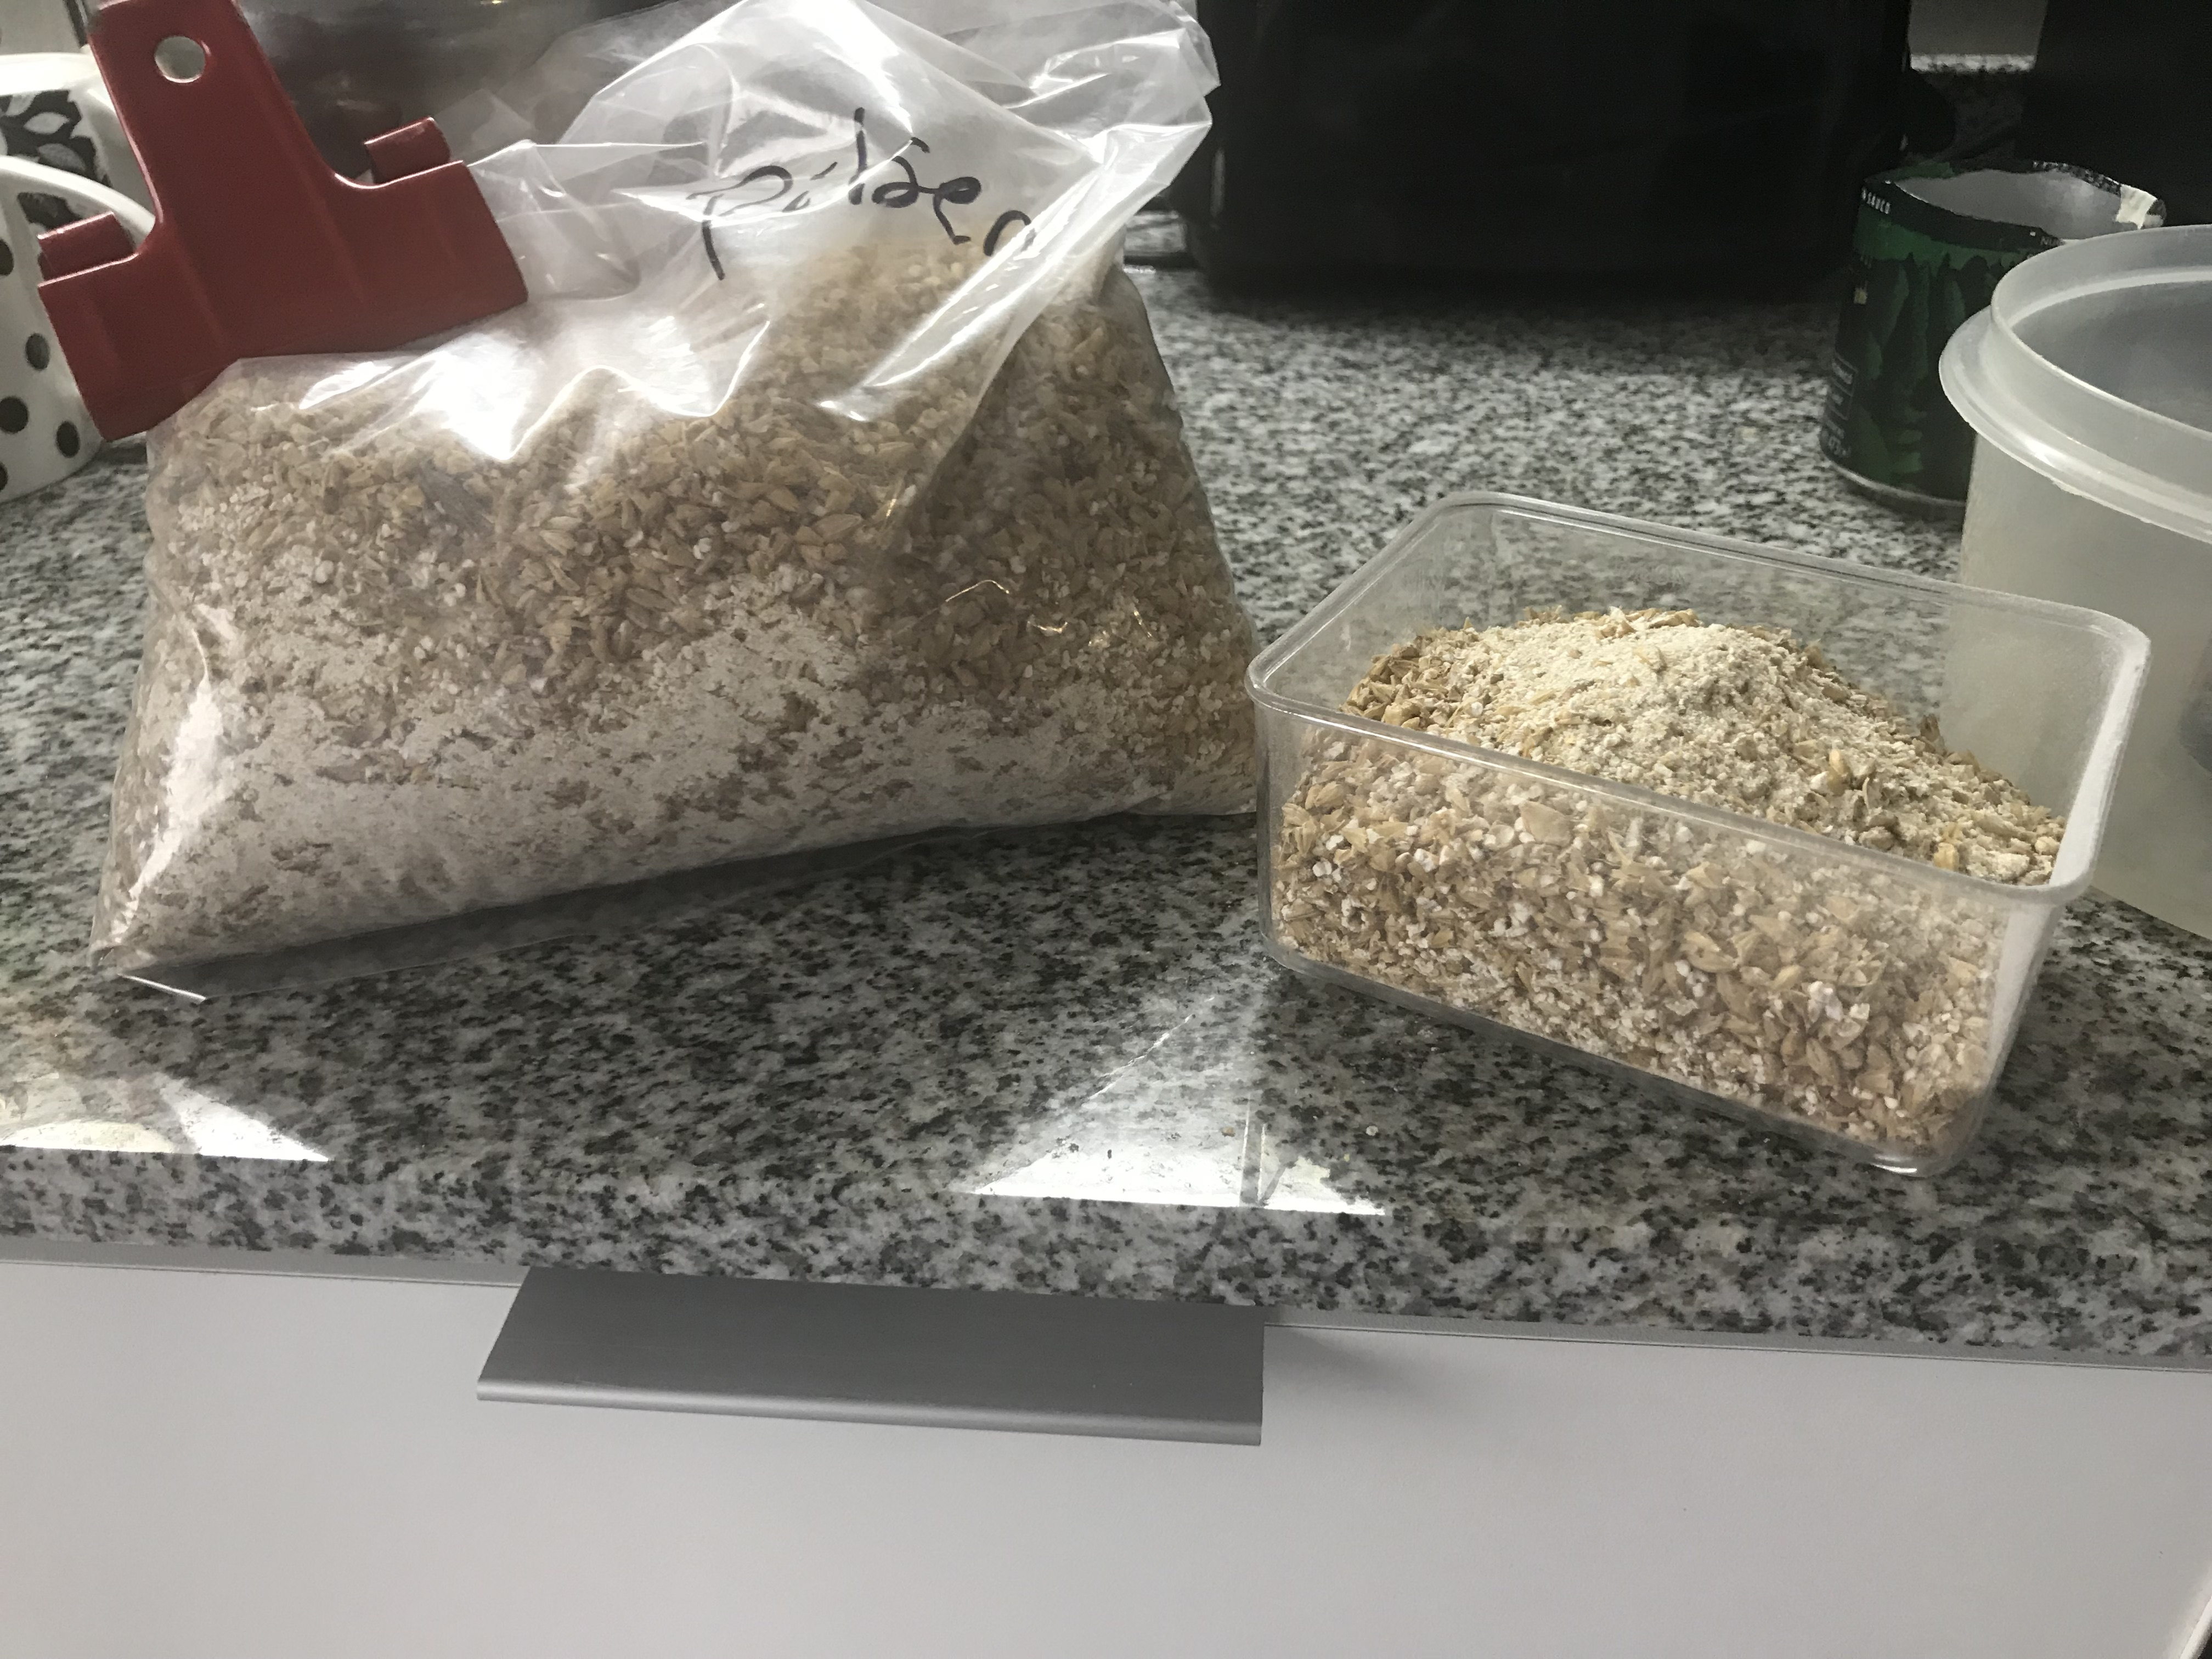
\includegraphics[scale=0.10]{Anexo/FotosExperimentos/P1.jpg}
        \captionof{figure}{Insumos}
        \label{fig:InsumosMalta}
    %\end{minipage}
        
    \begin{figure}
        \centering
        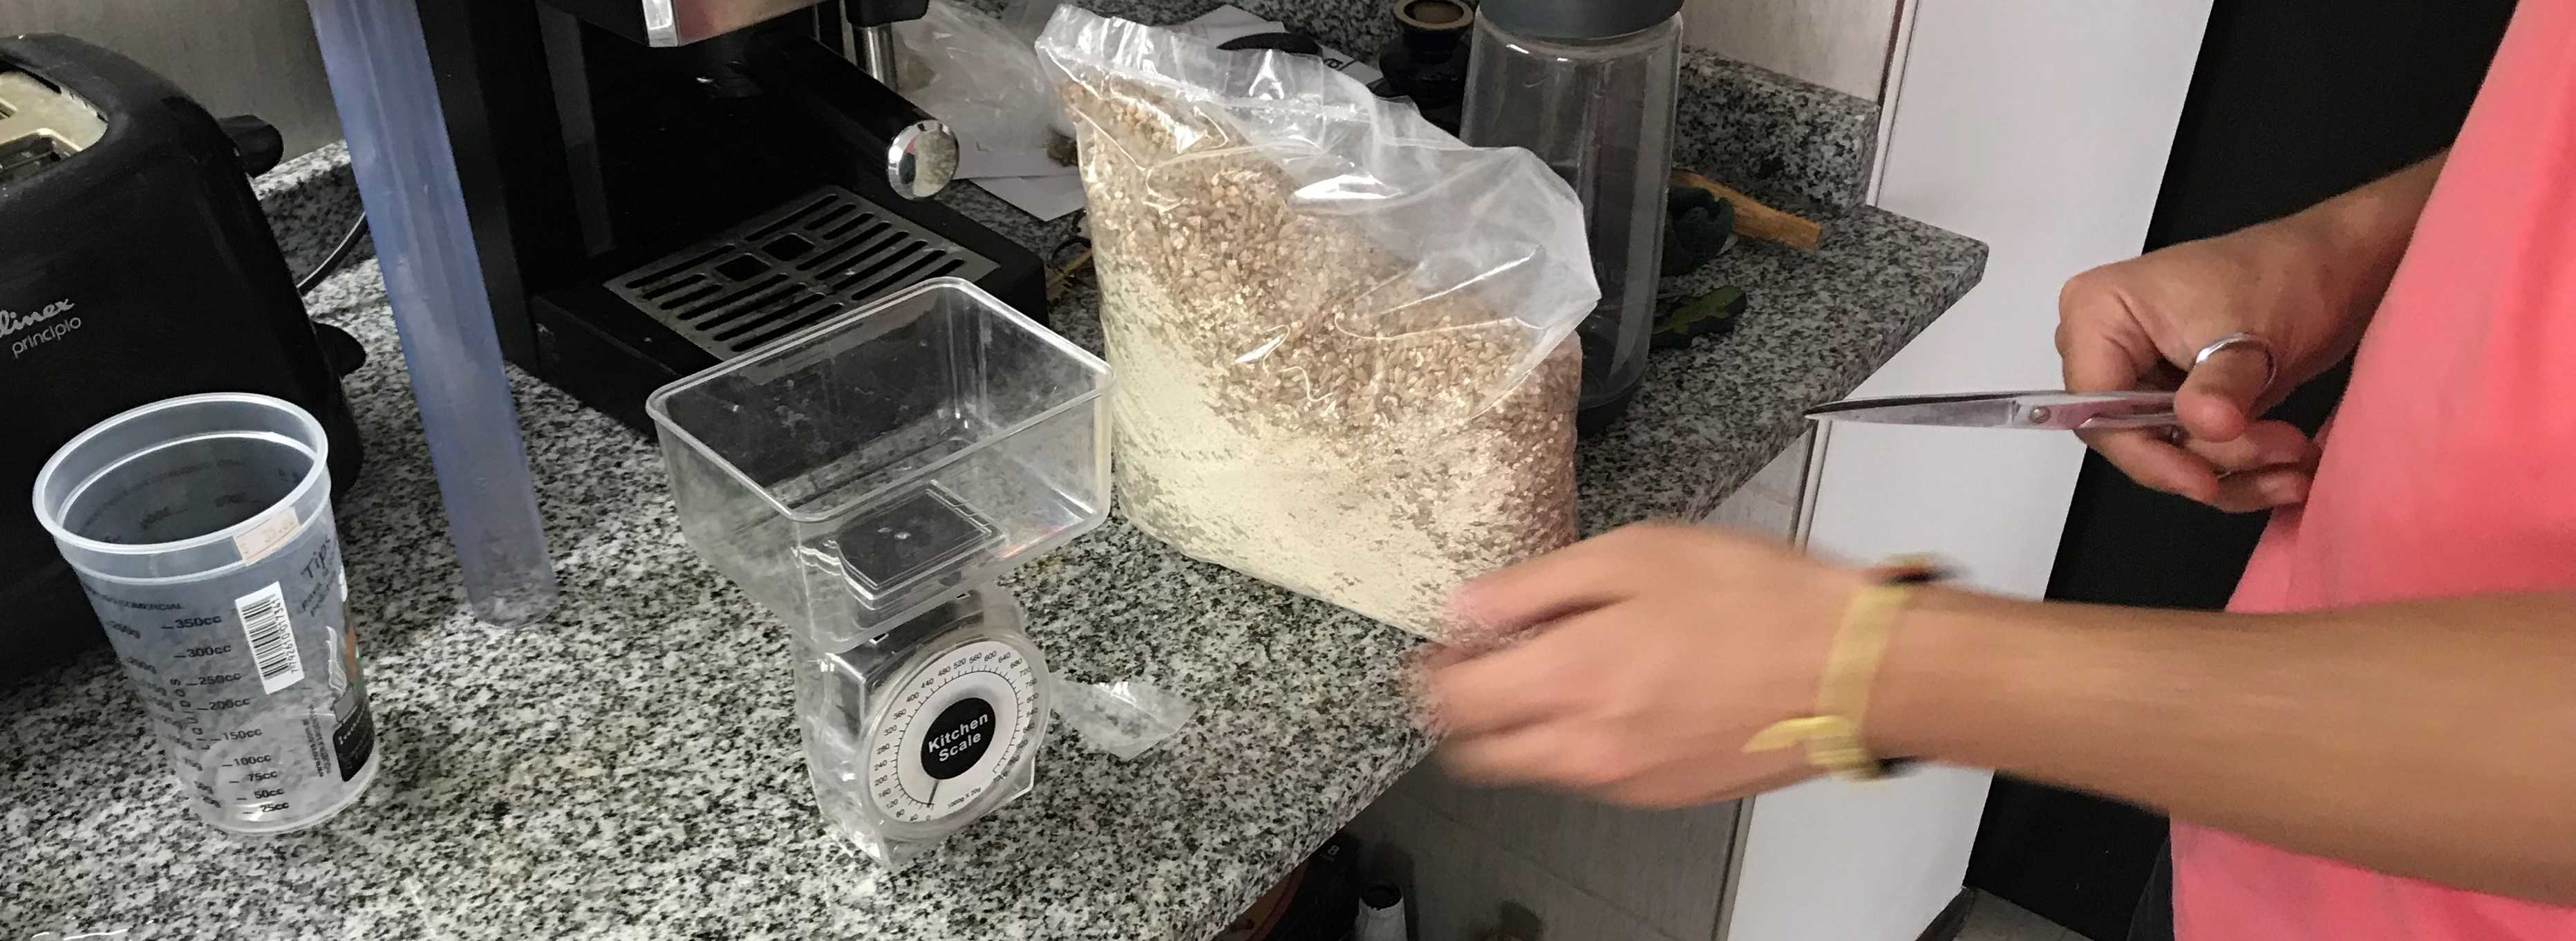
\includegraphics[scale=0.10]{Anexo/FotosExperimentos/P2.jpg}
        \captionof{figure}{Fragmentación de insumos}
        \label{fig:FragInsumos}
    \end{figure}
        
    \begin{figure}
        \centering
        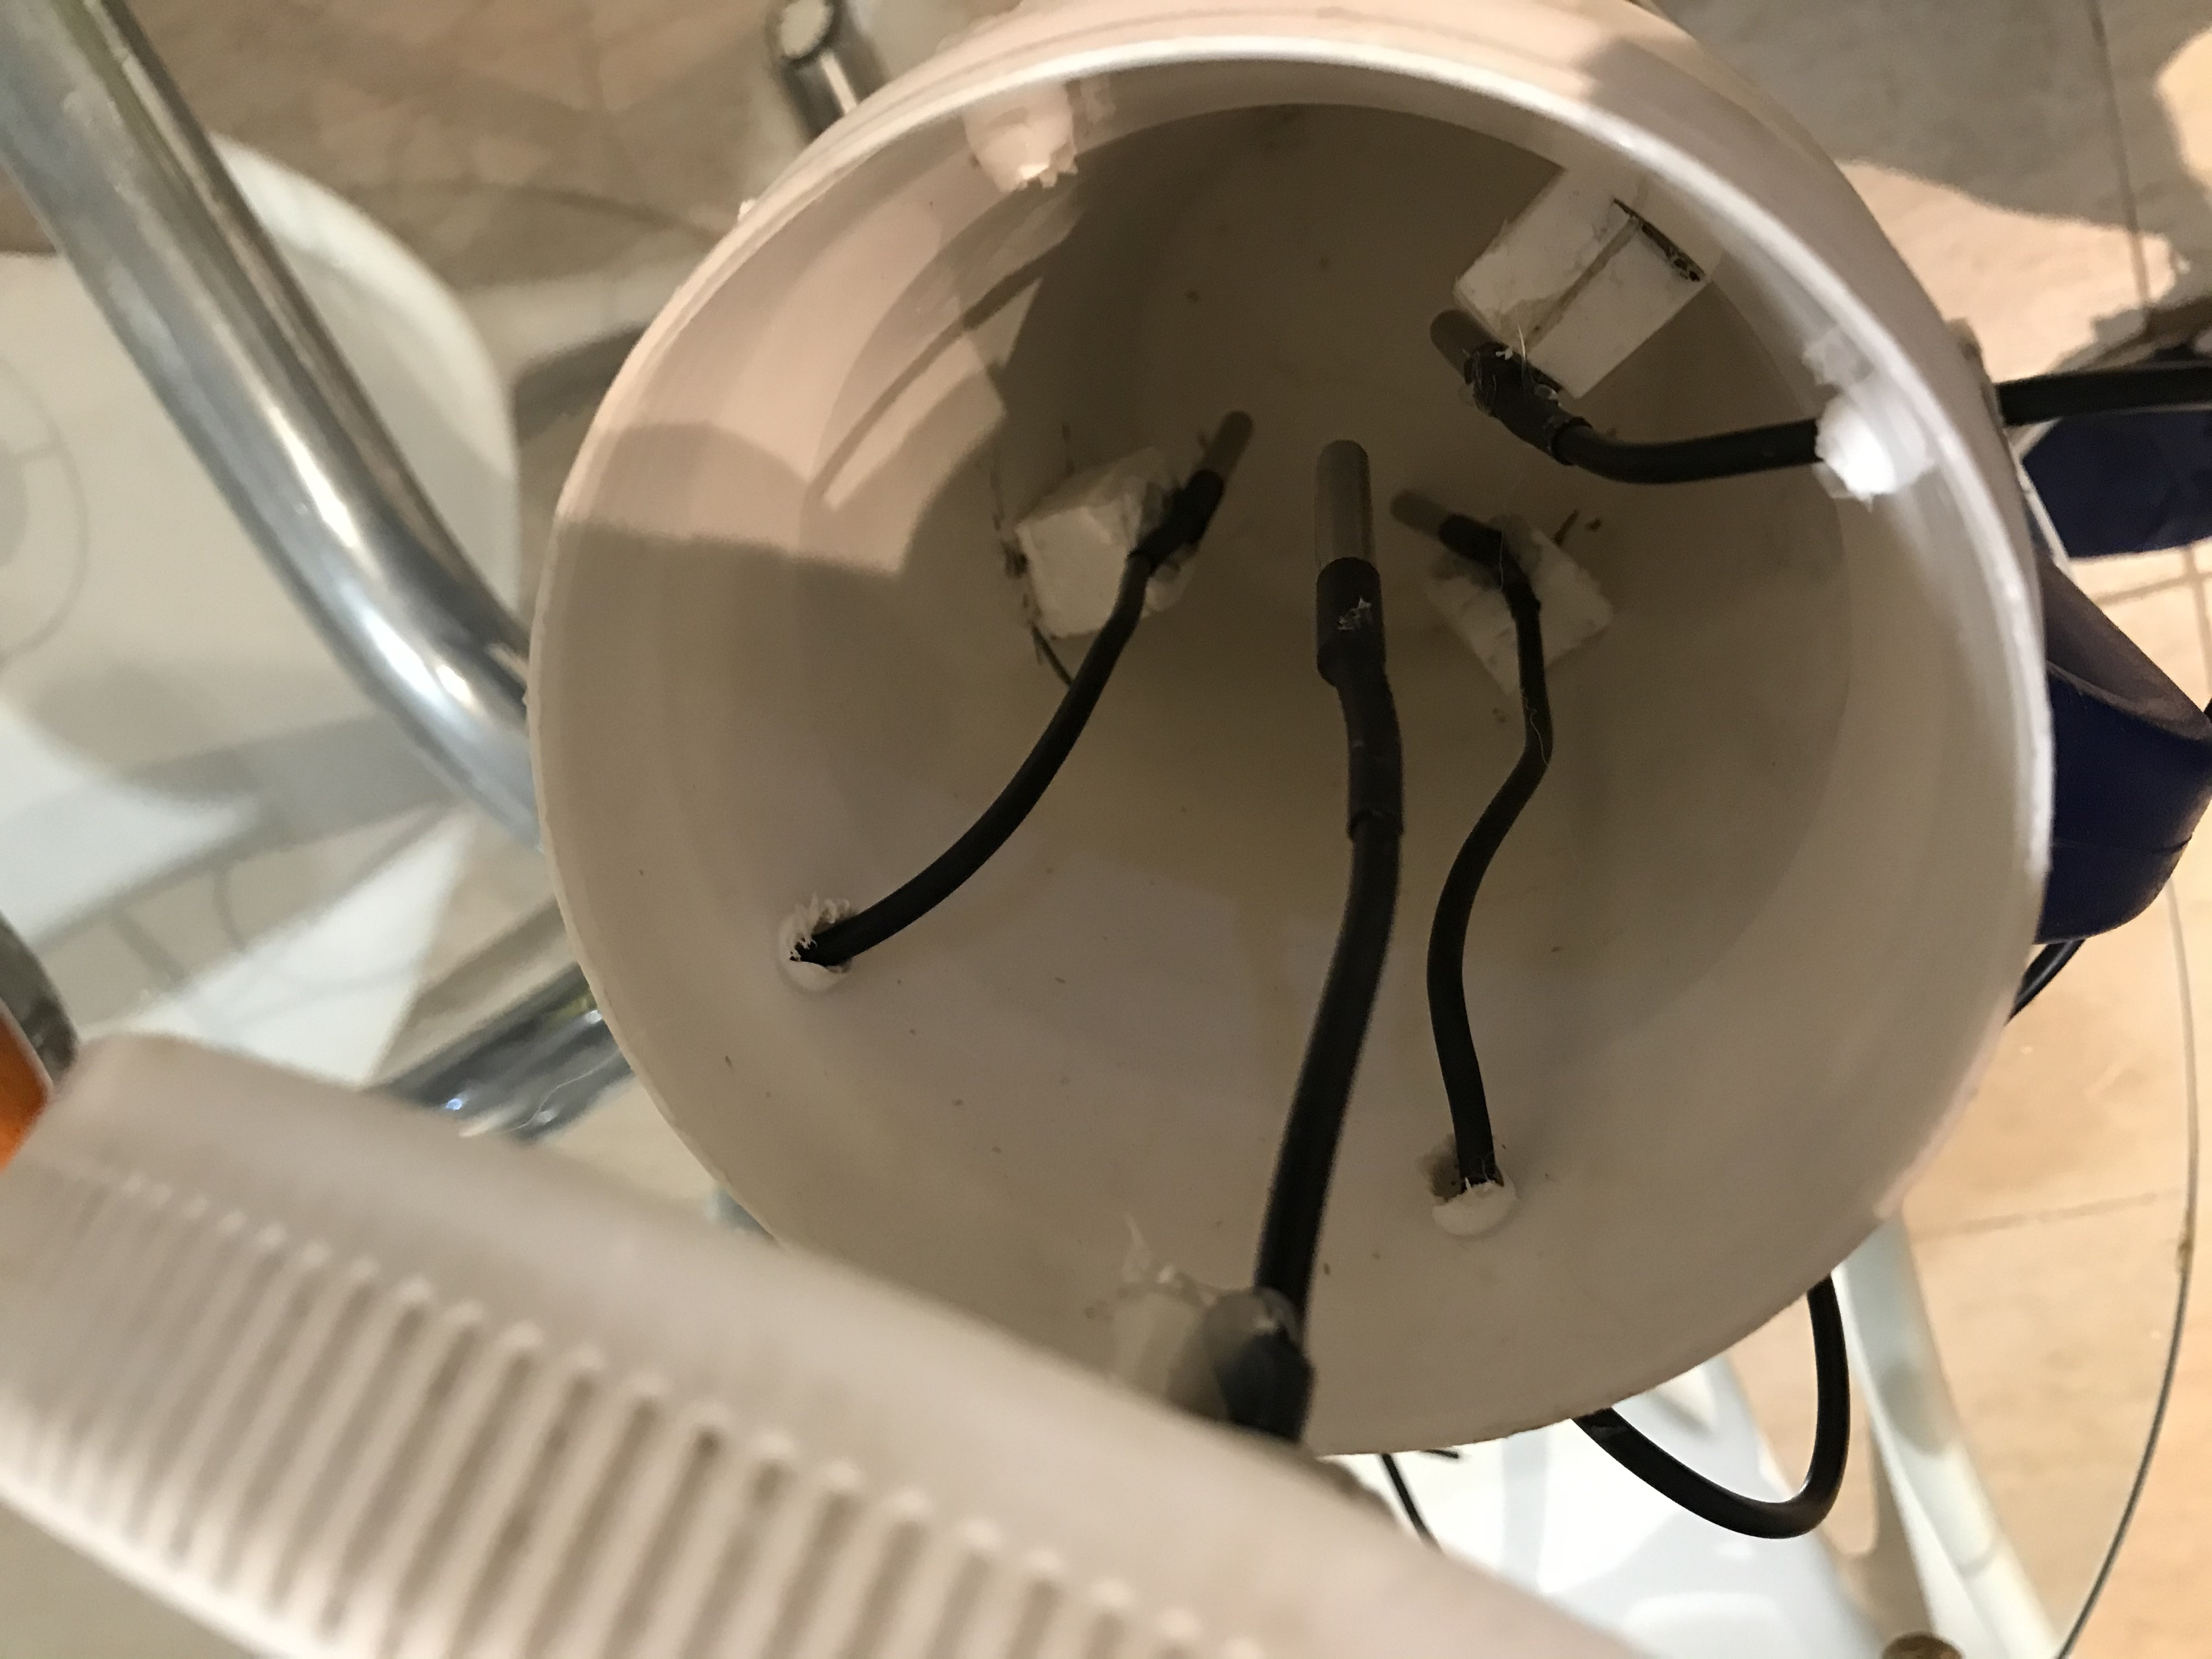
\includegraphics[scale=0.10]{Anexo/FotosExperimentos/tanque-nuevoP3.jpg}
        \captionof{figure}{Interior del termo}
        \label{fig:ConstrucMacerador}
    \end{figure}
    
    \begin{figure}
        \centering
        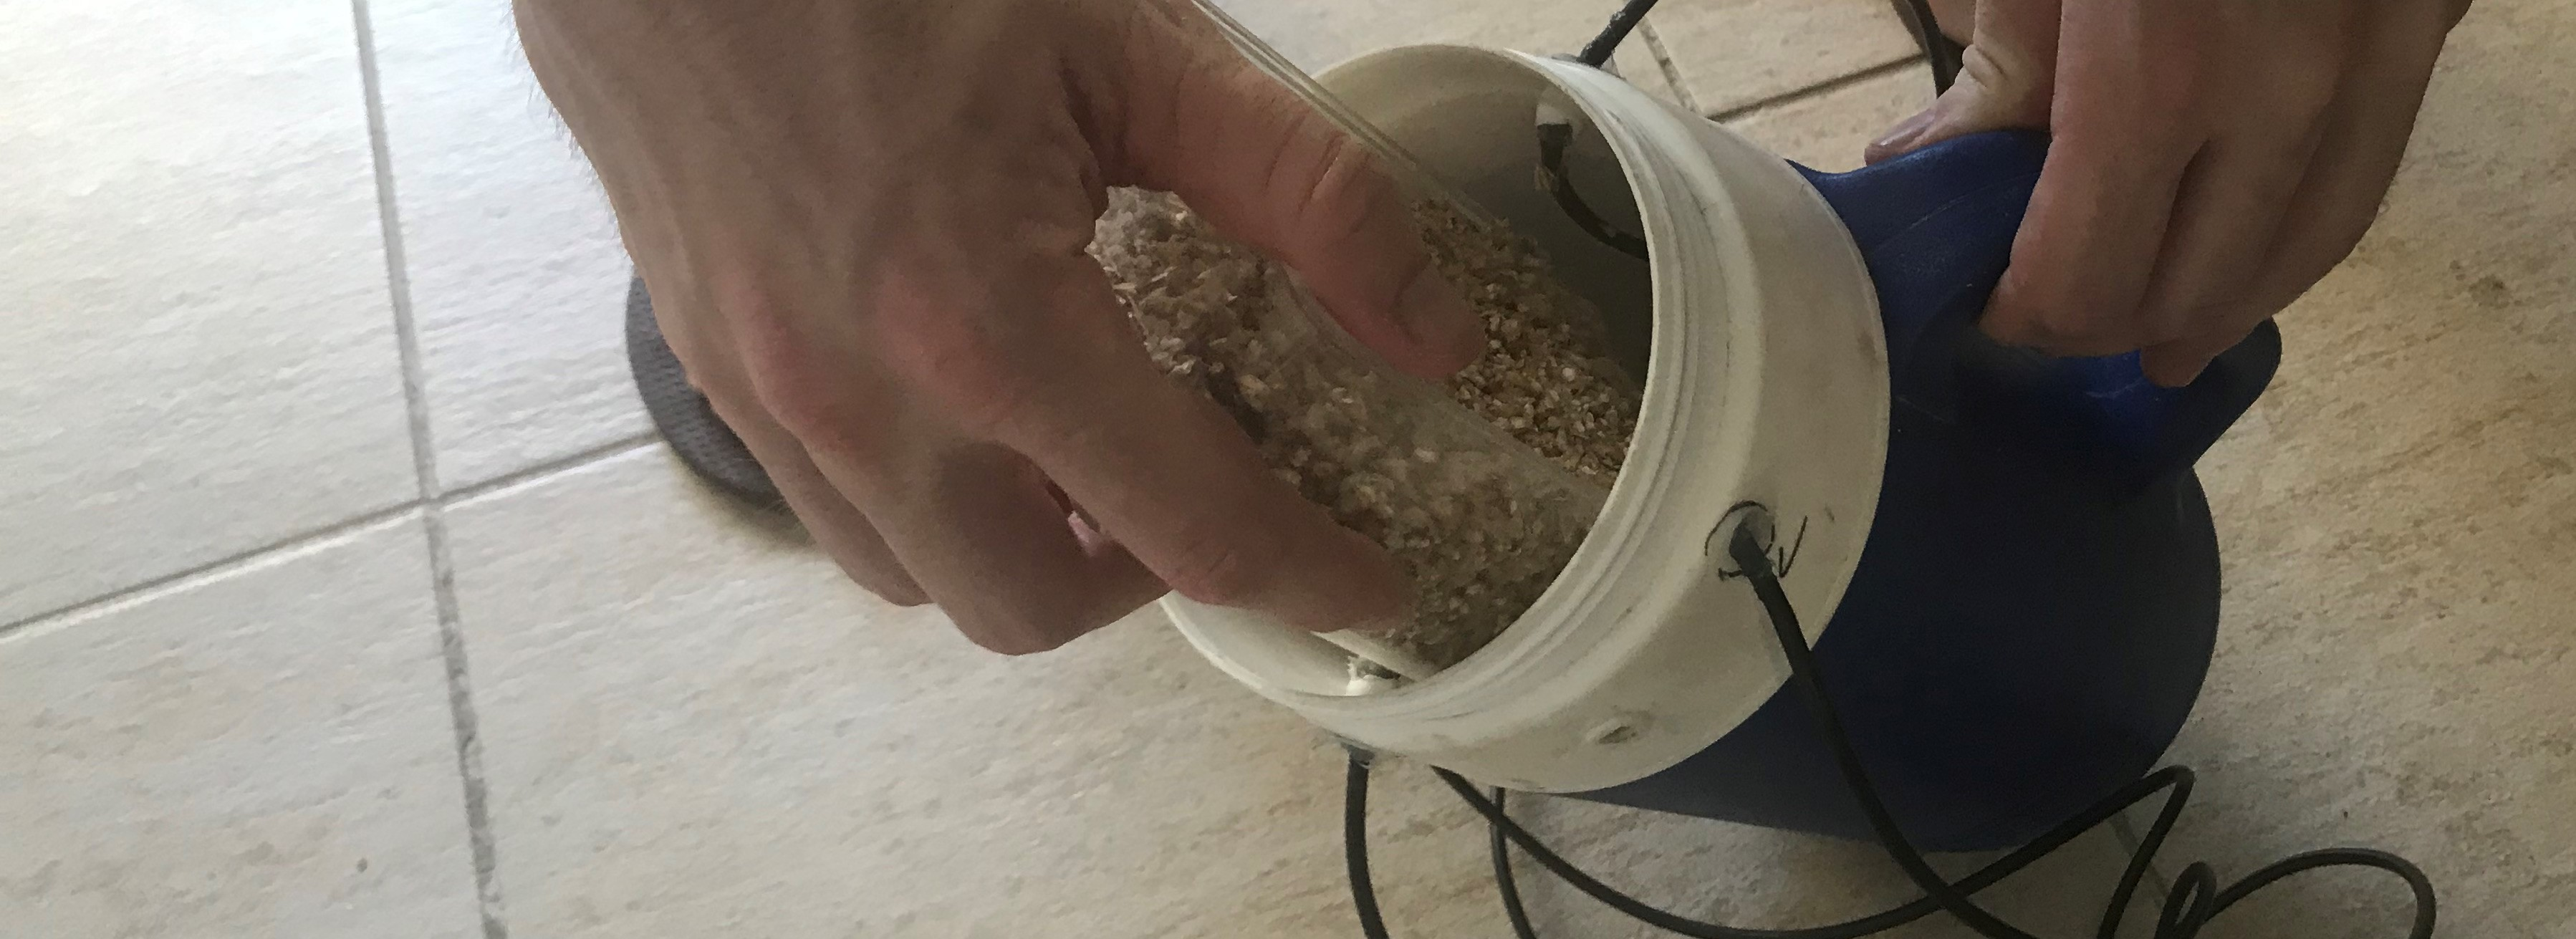
\includegraphics[scale=0.10]{Anexo/FotosExperimentos/P4.jpg}
        \captionof{figure}{Incorporación de insumos al macerador}
        \label{fig:IncorpInsumos}
    \end{figure}
    
    \begin{figure}
        \centering
        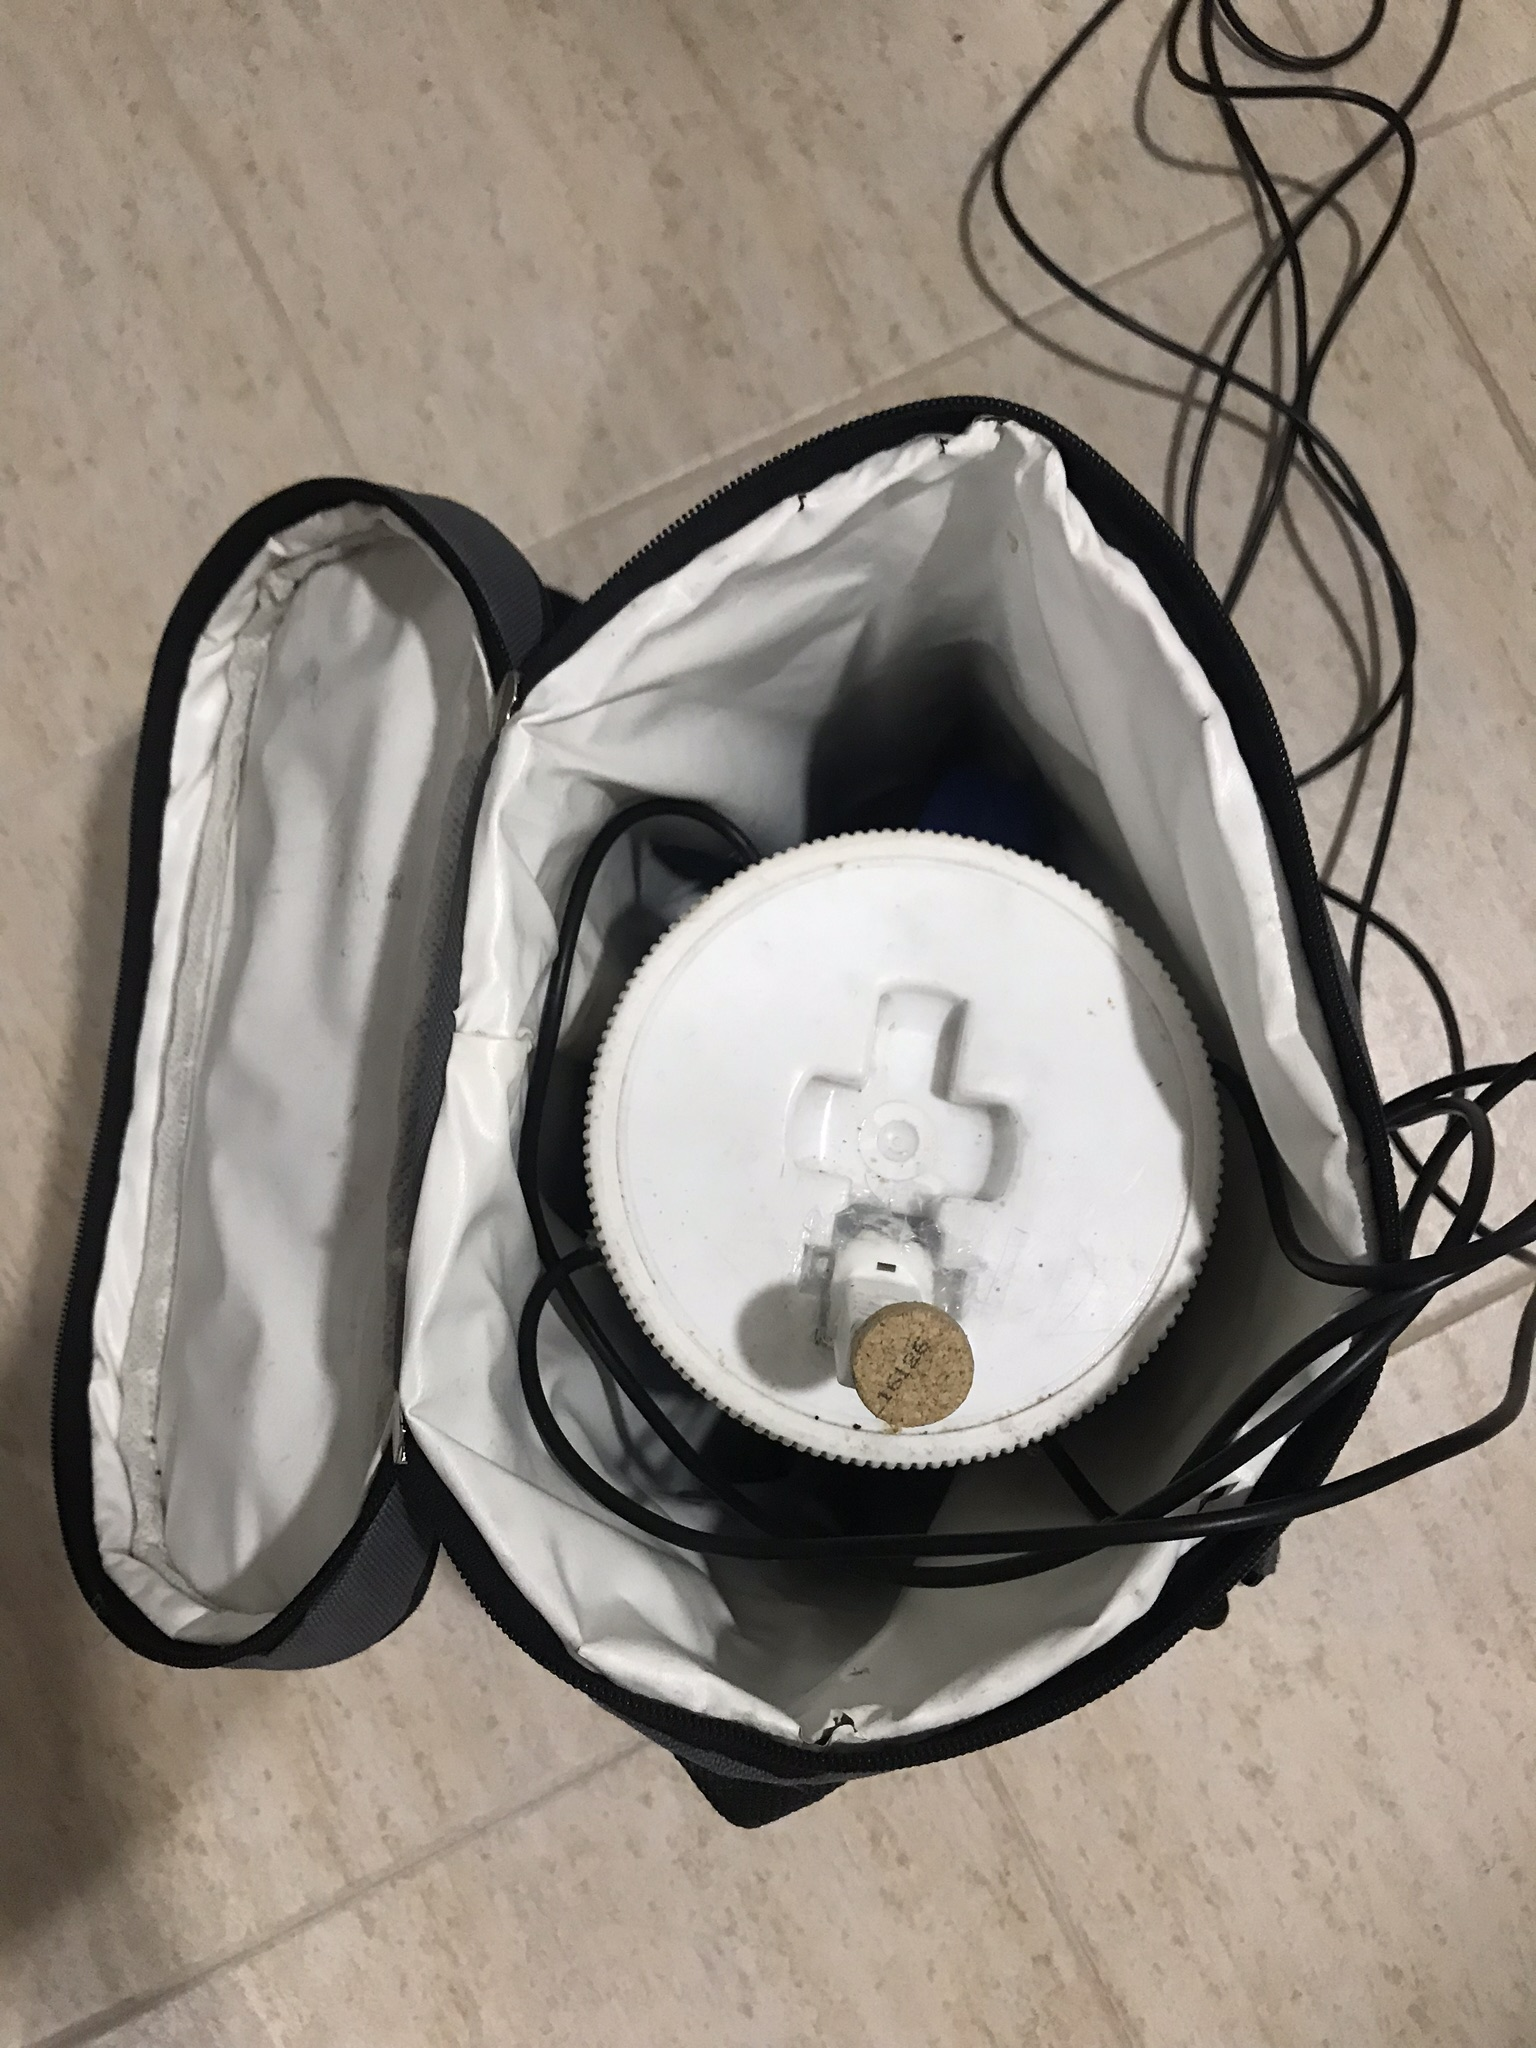
\includegraphics[scale=0.10]{Anexo/FotosExperimentos/P5.jpeg}
        \captionof{figure}{Aislamiento térmico}
        \label{fig:ConstrucAislamTerm}
    \end{figure}
    
    \begin{figure}
        \centering
        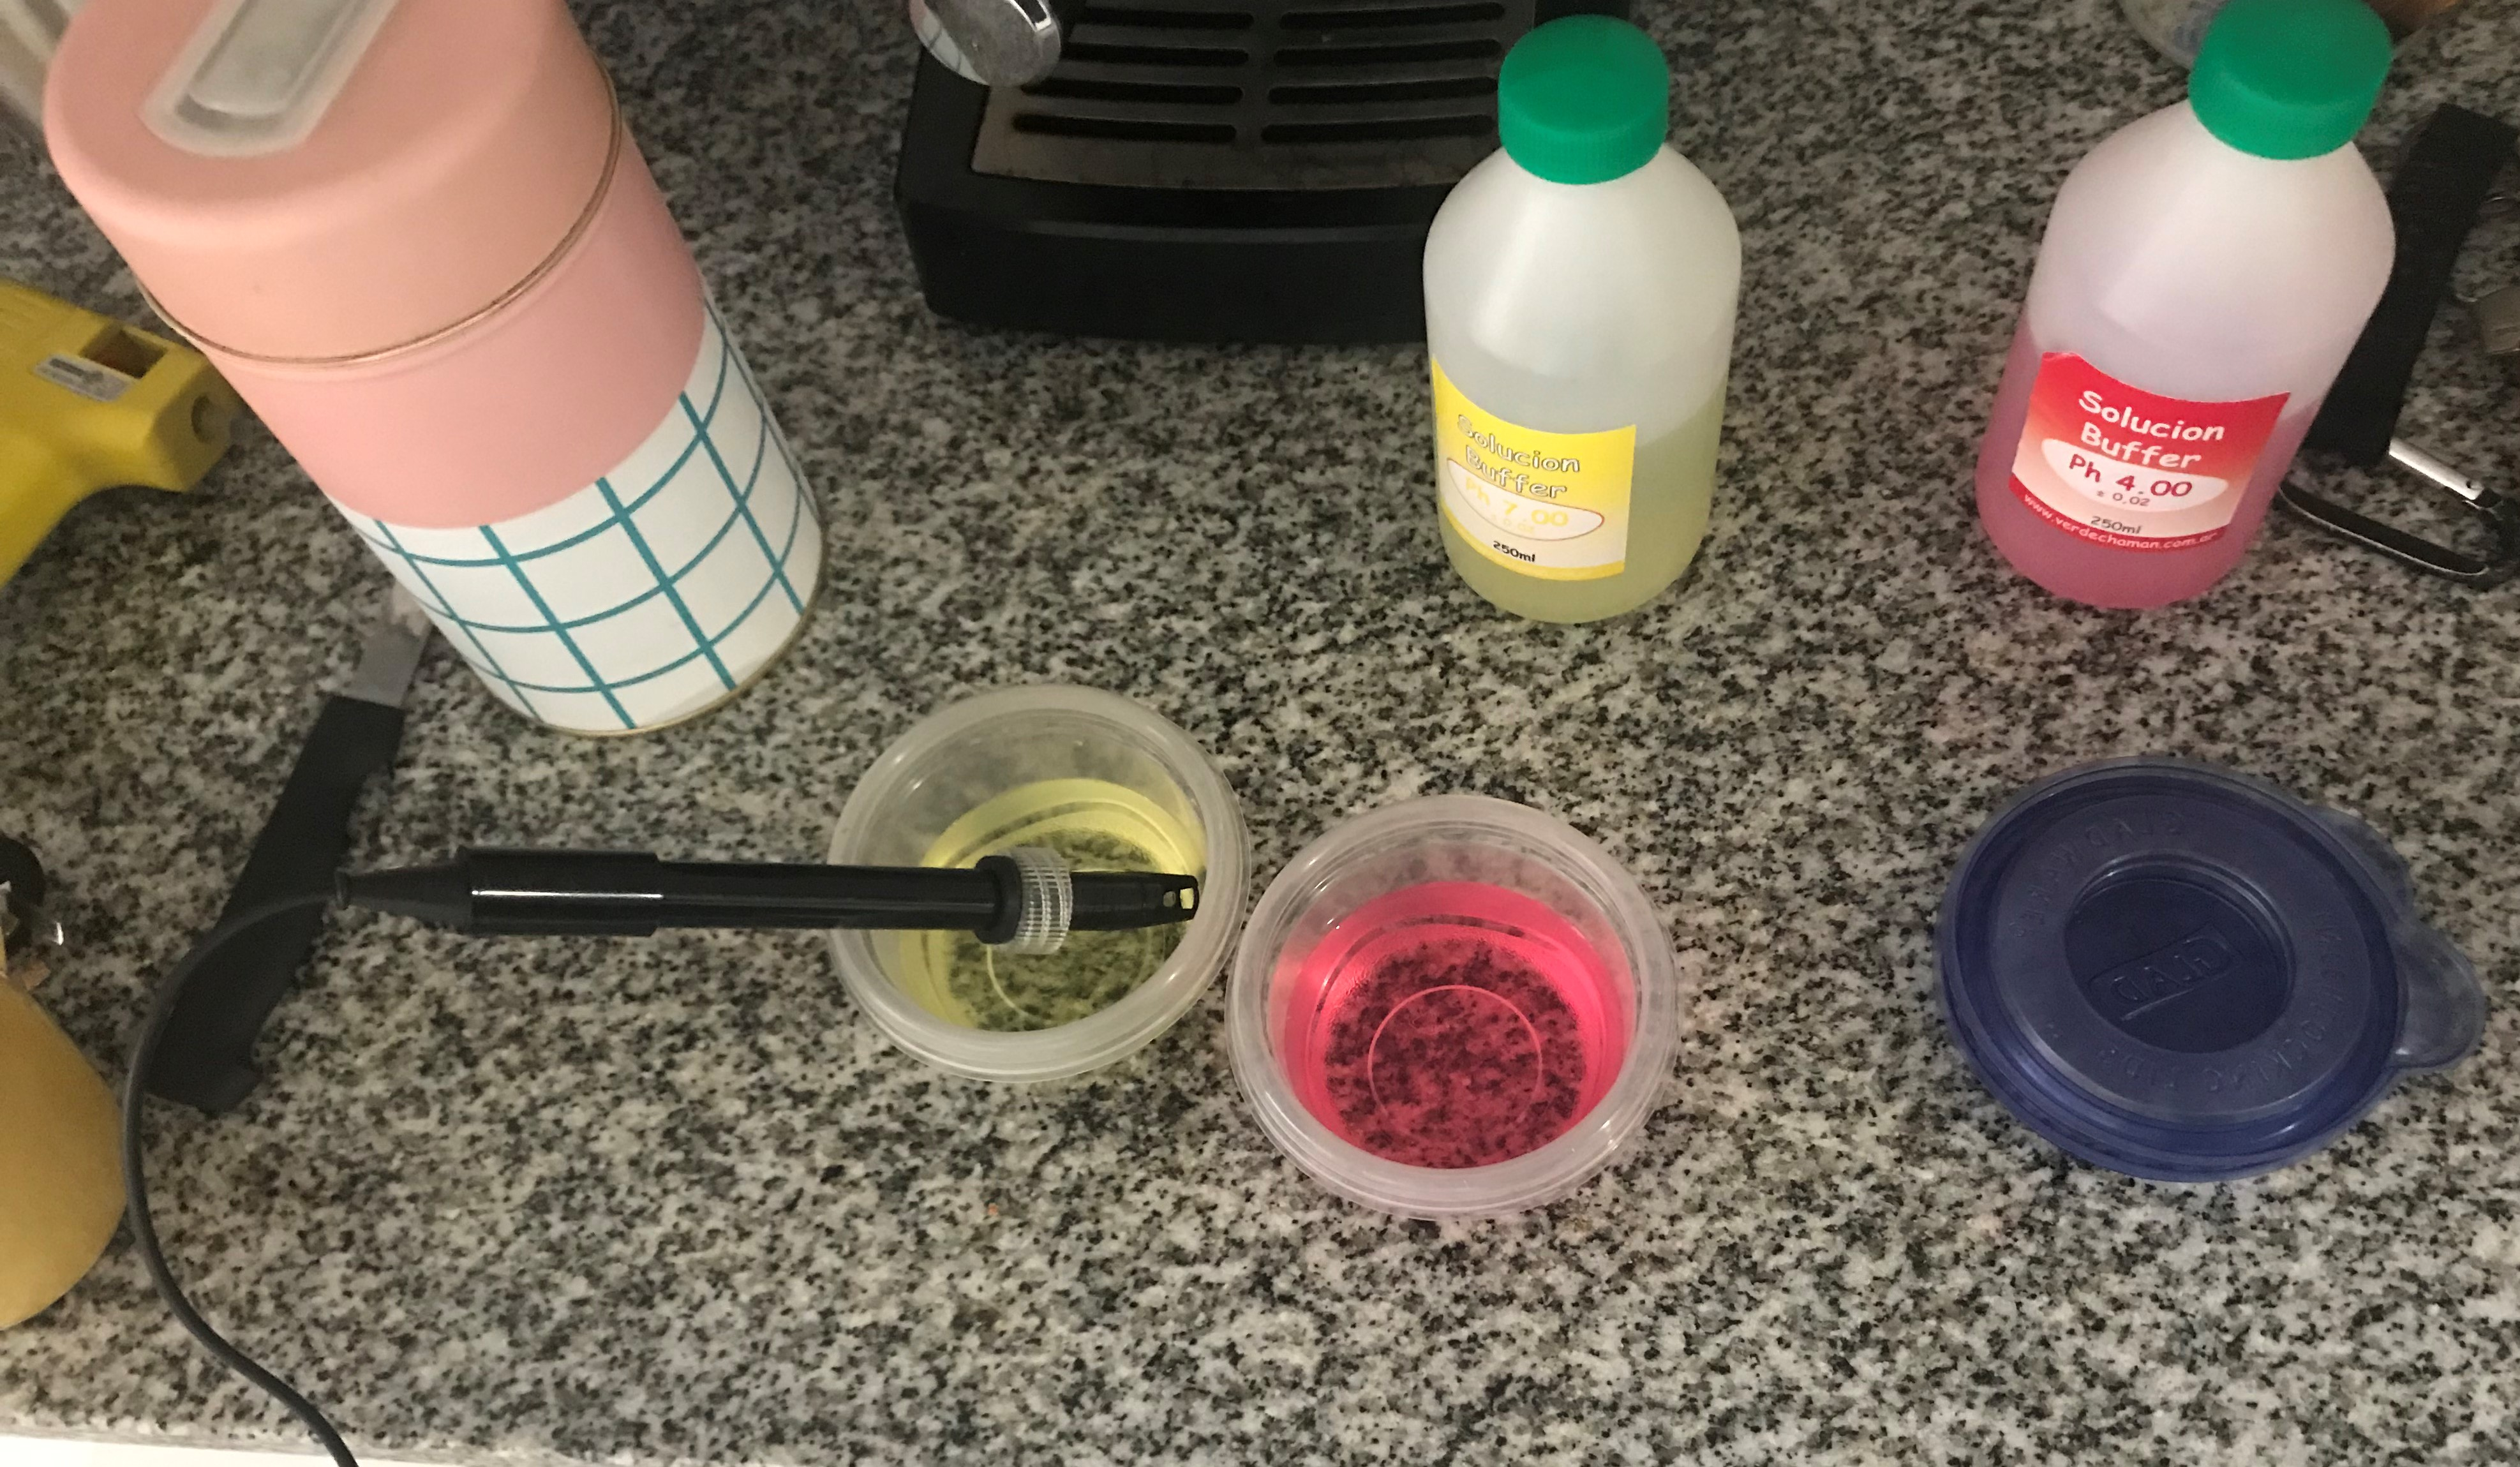
\includegraphics[scale=0.10]{Anexo/FotosExperimentos/P6.jpg}
        \captionof{figure}{Calibración del sensor de pH}
        \label{fig:CalibrPhimetro}
    \end{figure}
        
    \begin{figure}
        \centering
        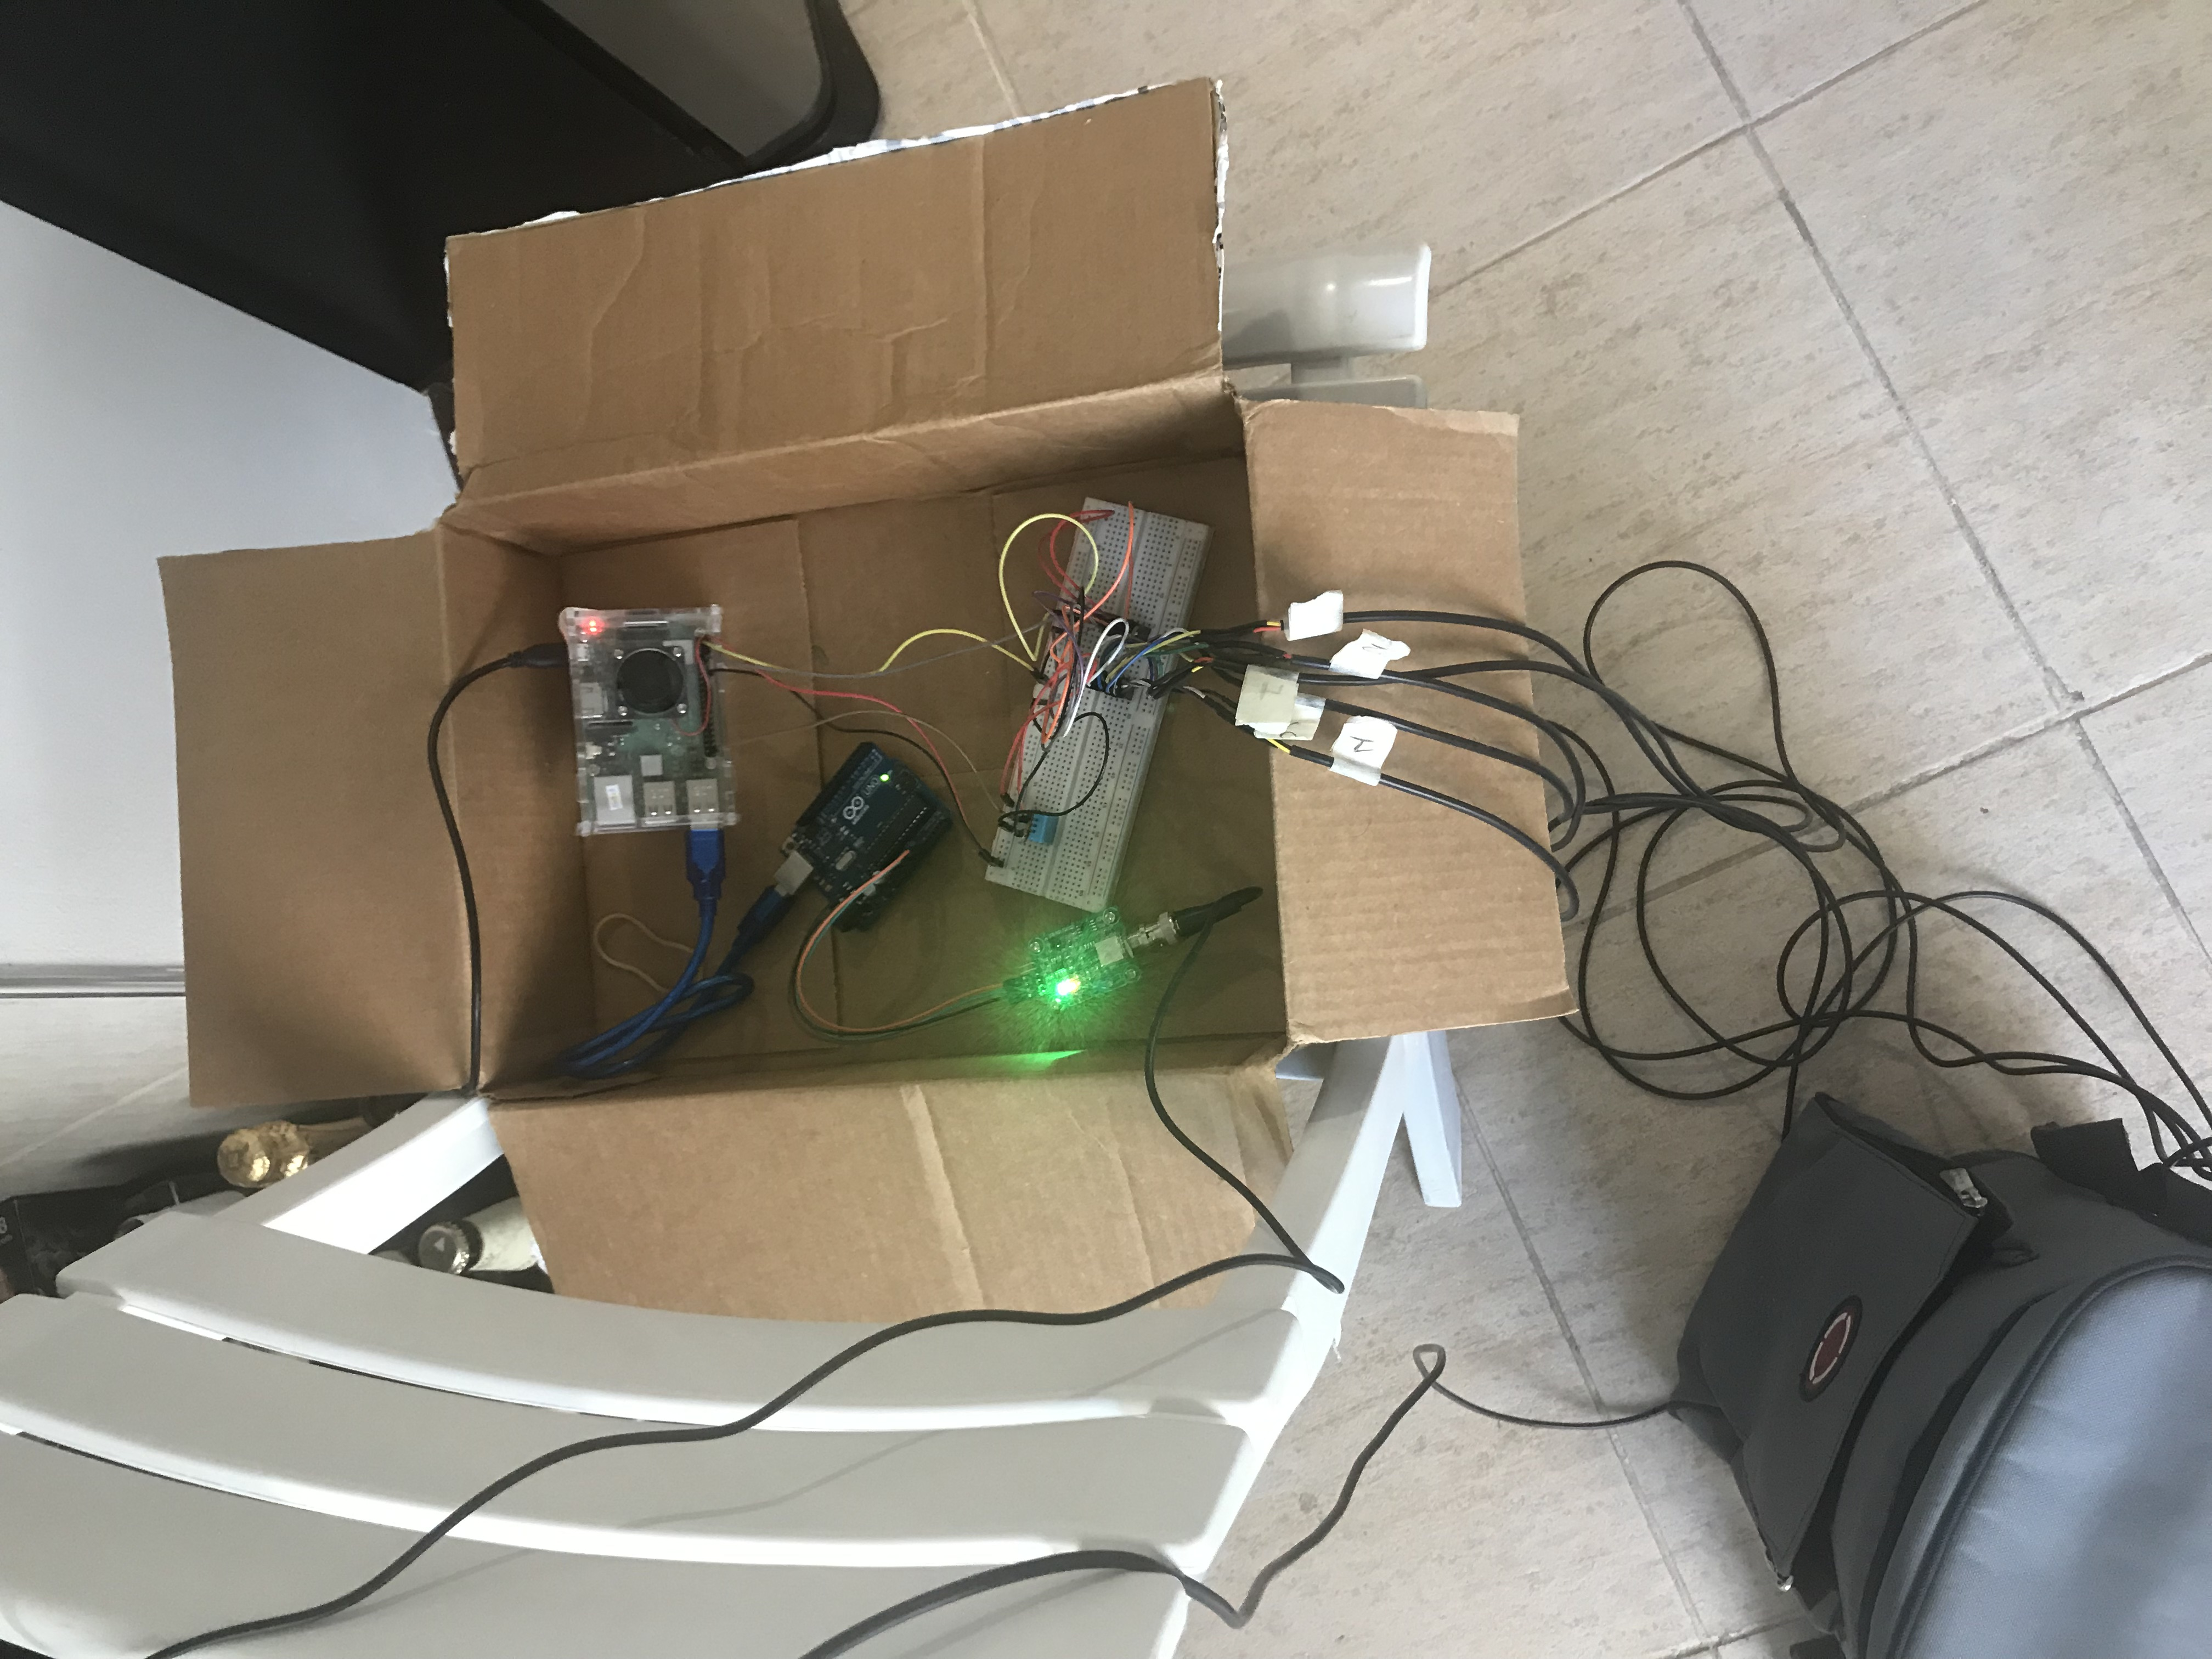
\includegraphics[scale=0.1]{Anexo/FotosExperimentos/P7.jpg}
        \captionof{figure}{Montaje del sistema}
        \label{fig:MontajeSist}
    \end{figure}
    
    \begin{figure}
        \centering
        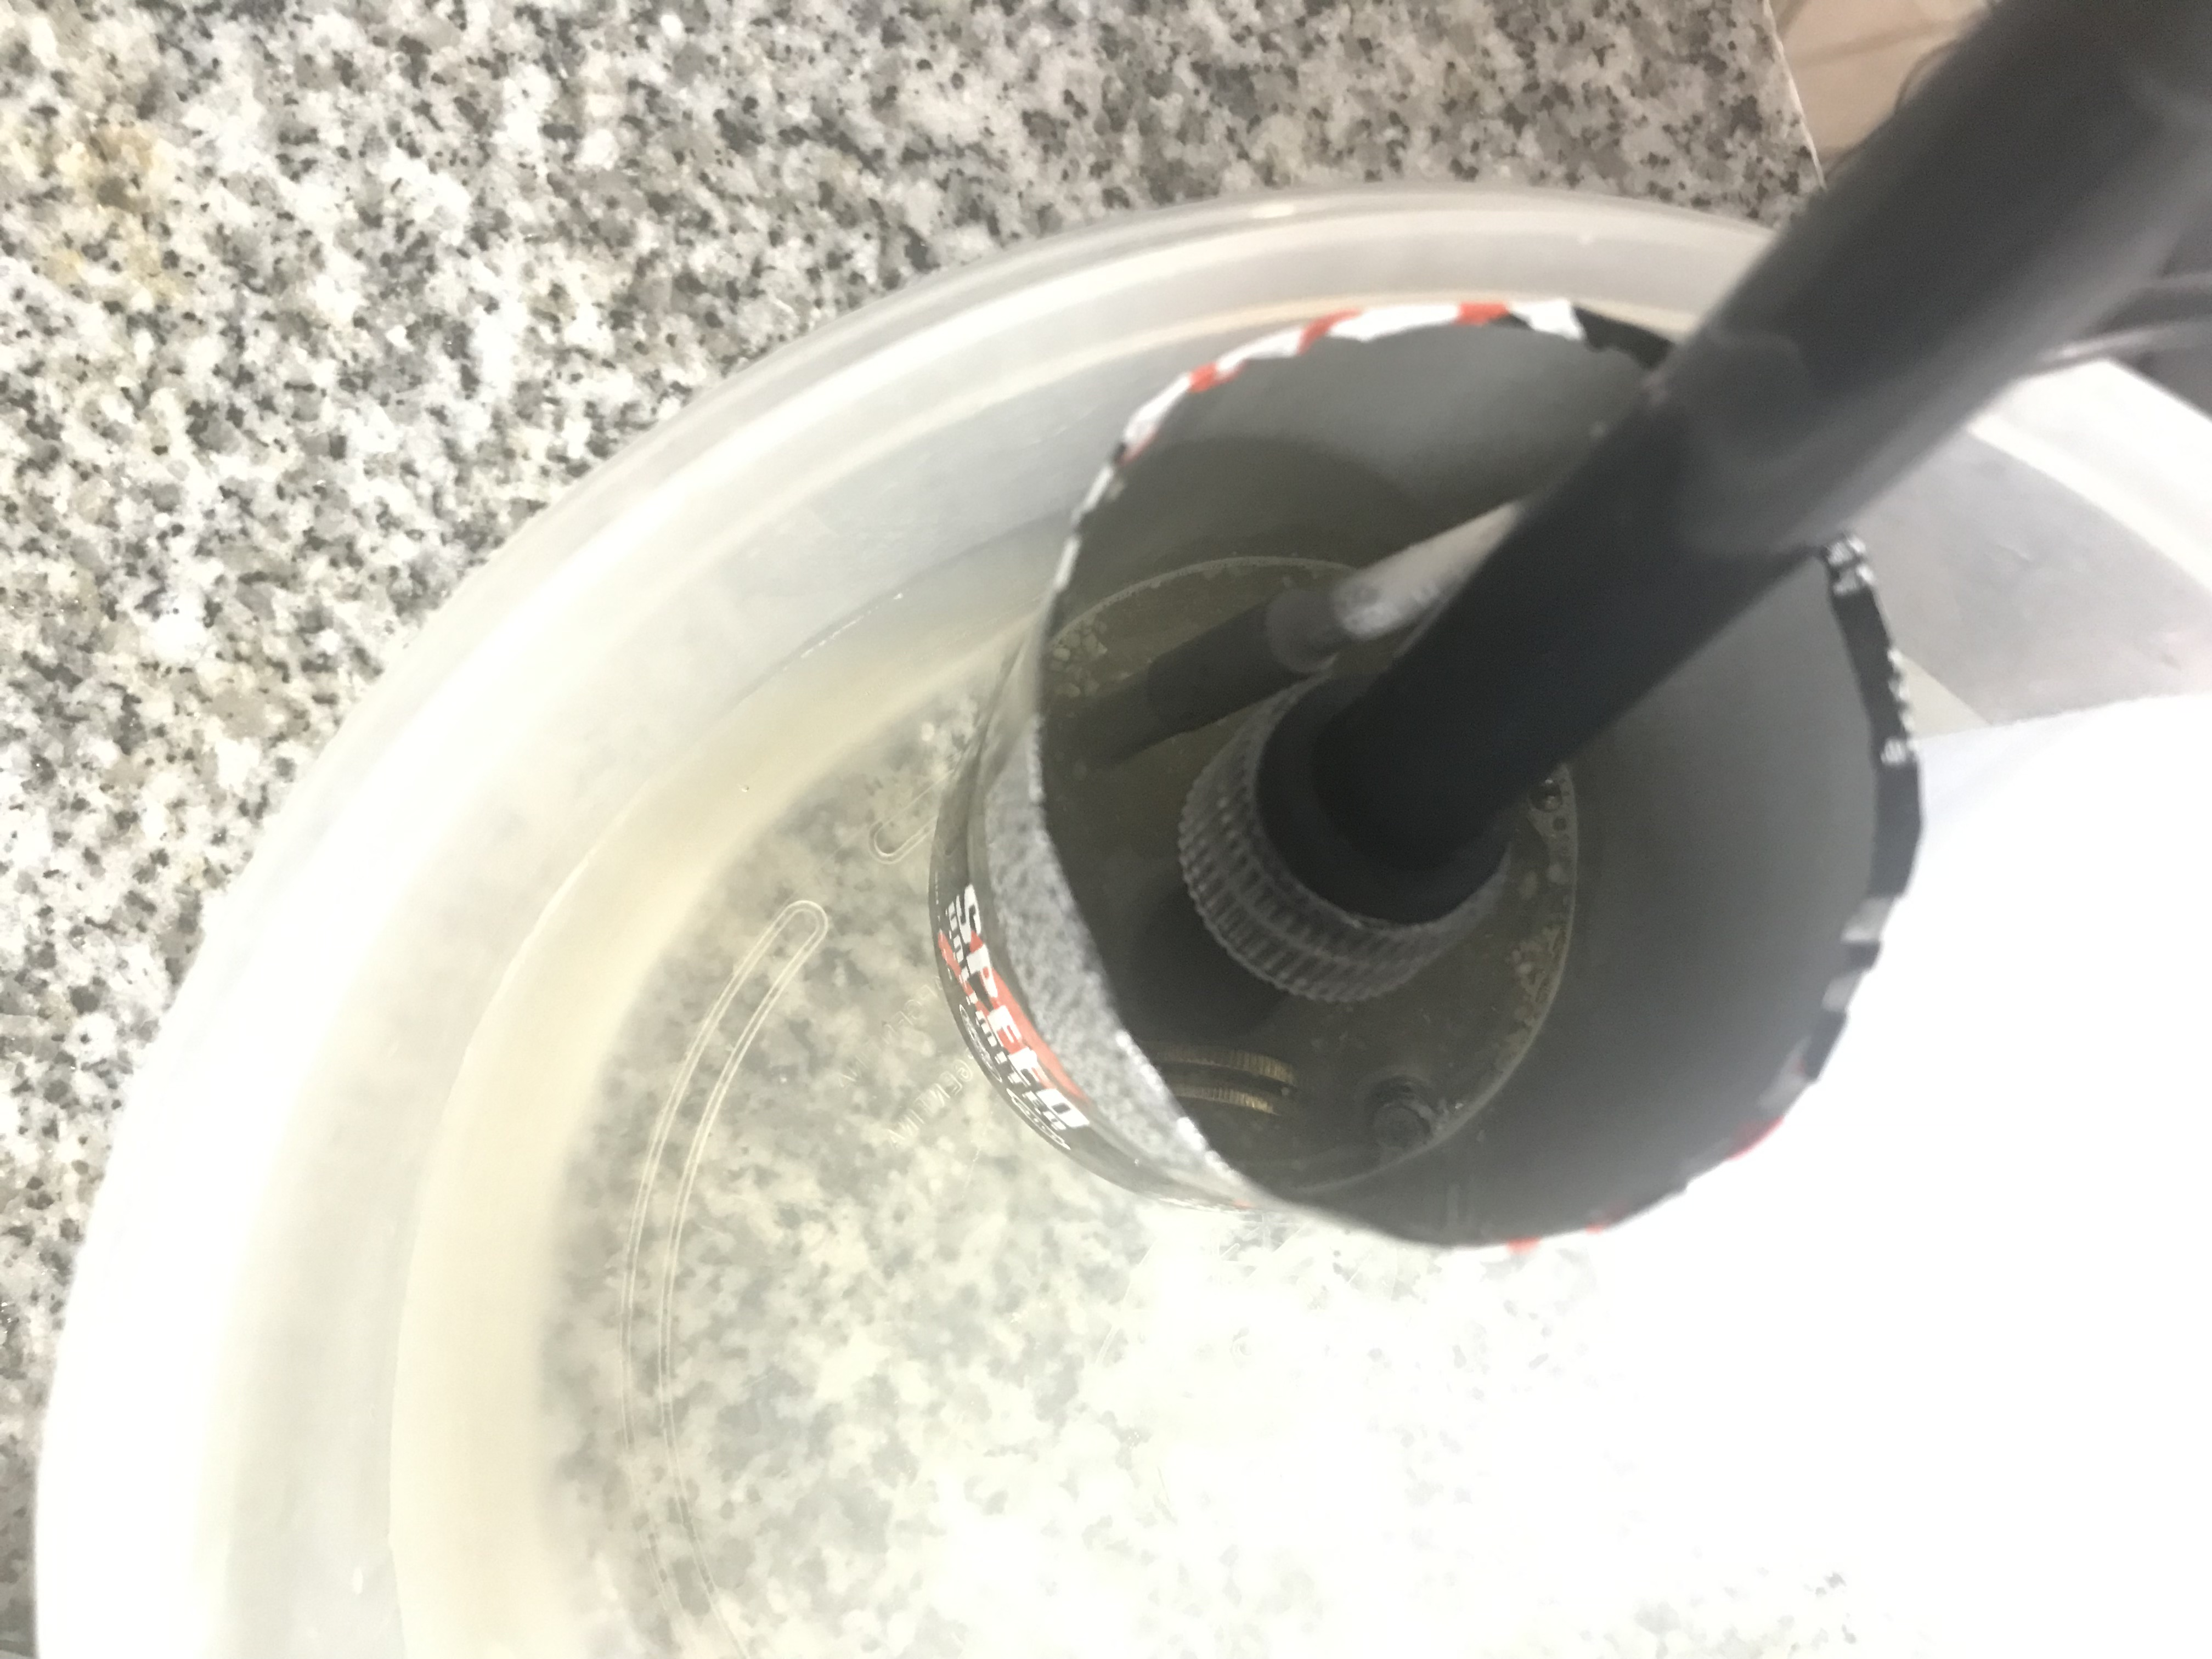
\includegraphics[scale=0.1]{Anexo/FotosExperimentos/P8.jpg}
        \captionof{figure}{Refrigerador de muestras}
        \label{fig:MedicPH}
    \end{figure}
        
    %\end{minipage}

    
\chapter{Mediciones pruebas de campo}
    \label{GraficasPruebasCampo}
    \begin{minipage}{\textwidth}
    \section{Pilsen Lager - Simple}
            %Experimento 1
        %\begin{minipage}{\textwidth}
            %\begin{figure}[H]
                \centering
                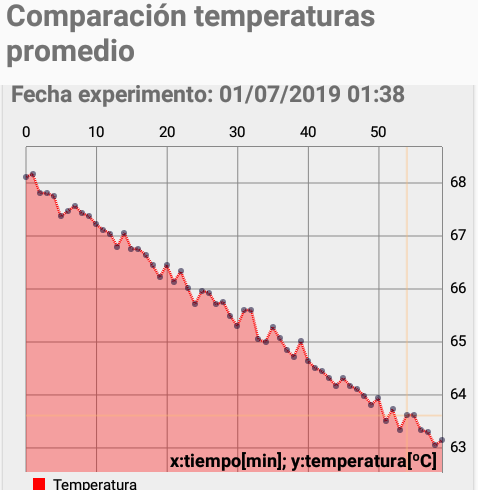
\includegraphics[scale=0.65]{Pruebas/SimpleExp1.jpg}
                \captionof{figure}{Maceración simple: Evolución de la temperatura durante las mediciones en experimento 1}
                \label{fig:SimpTempExp1}
            %\end{figure}
    \end{minipage}     
            %Experimento 2
            \begin{figure}[H]
                \centering
                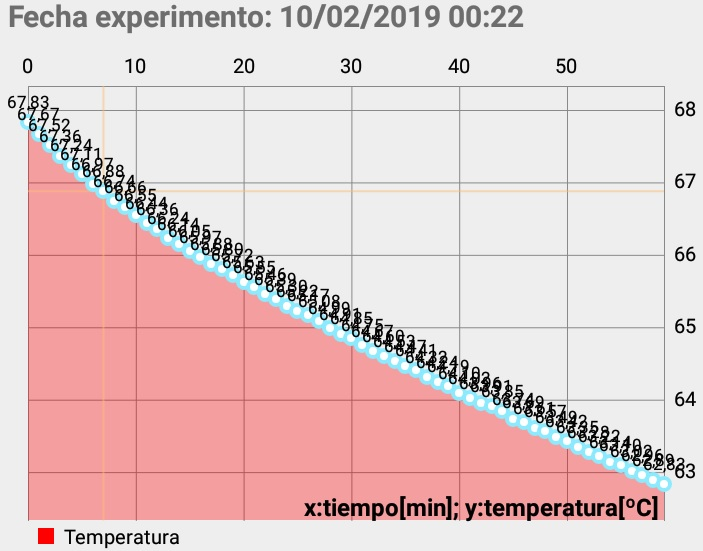
\includegraphics[scale=0.65]{Pruebas/SimpleExp2.jpg}
                \captionof{figure}{Maceración simple: Evolución de la temperatura durante las mediciones en experimento 2}
                \label{fig:SimpTempExp2}
            \end{figure}

        %\end{minipage}
        
        %\begin{minipage}{\textwidth}
                   
           %Experimento 3
            \begin{figure}[H]
                \centering
                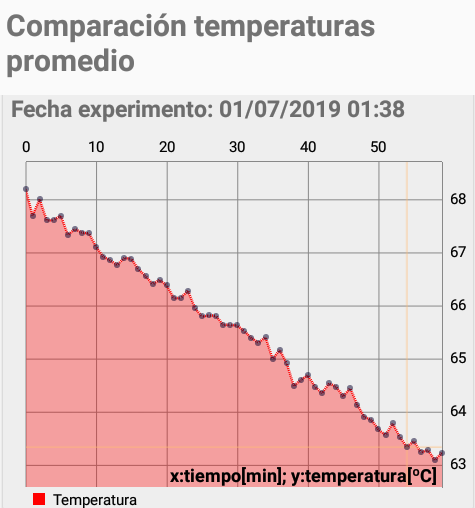
\includegraphics[scale=0.65]{Pruebas/SimpleExp3.jpg}
                \captionof{figure}{Maceración simple: Evolución de la temperatura durante las mediciones en experimento 3}
                \label{fig:SimpTempExp3}
            \end{figure}
        
            %Valores generales/promedio
            \begin{figure}[H]
                \centering
                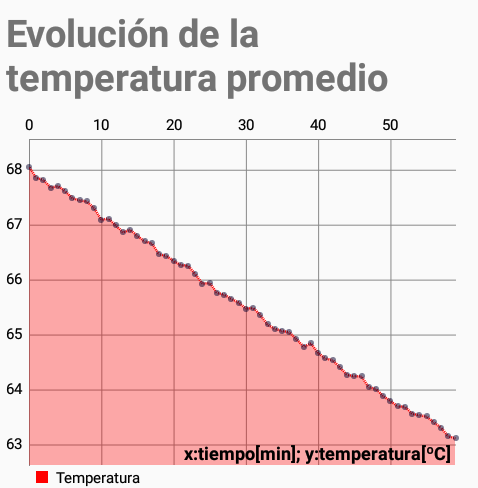
\includegraphics[scale=0.65]{Pruebas/SimpleEvolTempProm.jpg}
                \captionof{figure}{Maceración simple: Evolución de la temperatura promedio de todos los Experimentos}
                \label{fig:SimpTempProm}
            \end{figure}
           
            \begin{figure}[H]
                \centering
                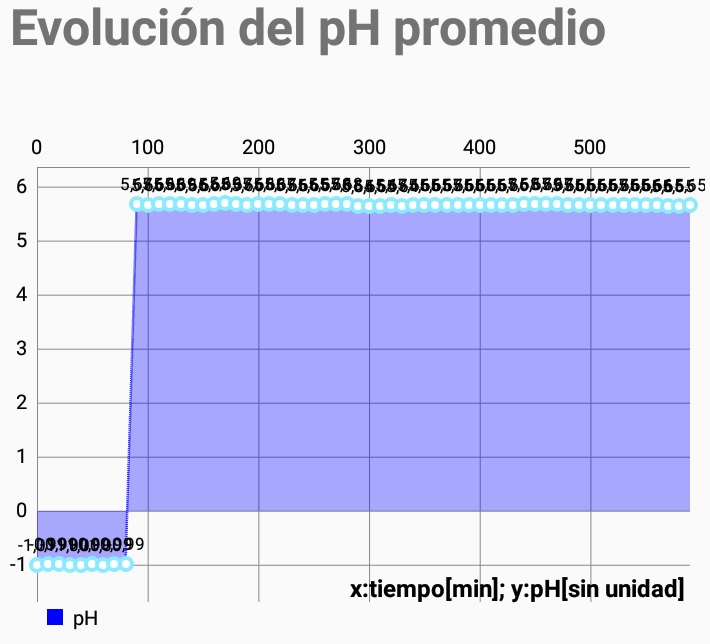
\includegraphics[scale=0.65]{Pruebas/SimpleEvolPHProm.jpg}
                \captionof{figure}{Maceración simple: Evolución del pH promedio de todos los Experimentos}
                \label{fig:SimpPHProm}
            \end{figure}

    \section{Pilsen Lager - Escalonada}
         %Experimento 1
            \begin{figure}[H]
                \centering
                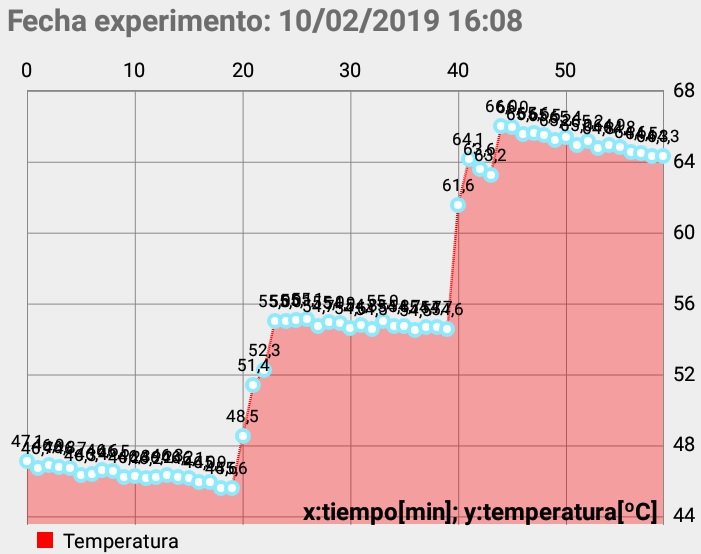
\includegraphics[scale=0.65]{Pruebas/EscalonadaExp1.jpg}
                \captionof{figure}{Maceración escalonada: Evolución de la temperatura durante las mediciones en experimento 1}
                \label{fig:EscExp1}
            \end{figure}
        %\end{minipage}
        
        
            \begin{figure}[H]
            %\begin{minipage}{\textwidth}    
                \centering
                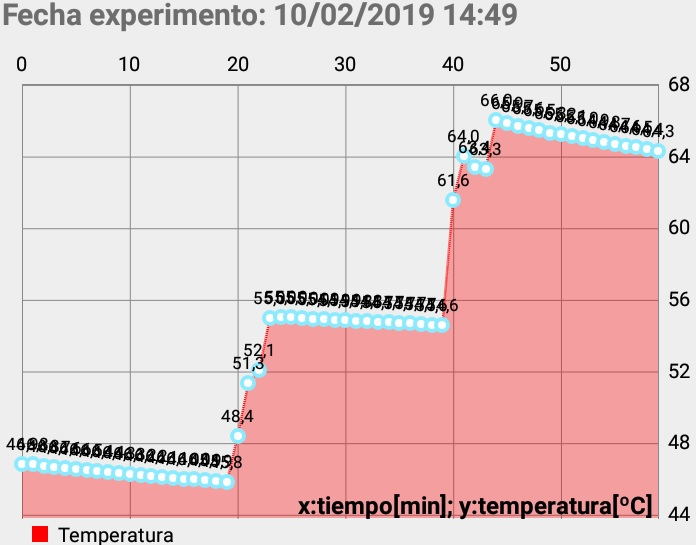
\includegraphics[scale=0.65]{Pruebas/EscalonadaExp2.jpg}
                \captionof{figure}{Maceración escalonada: Evolución de la temperatura durante las mediciones en experimento 2}
                \label{fig:EscExp2}
            \end{figure}
                
            \begin{figure}[H]    
                \centering
                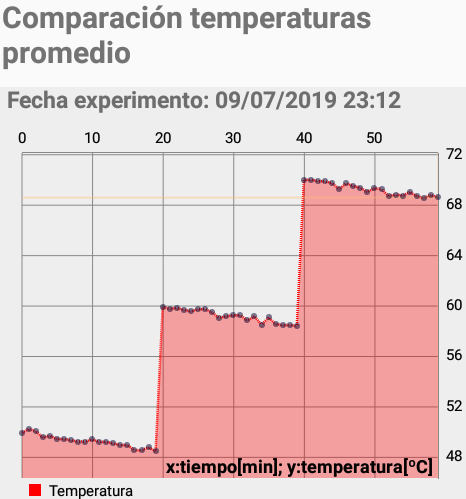
\includegraphics[scale=0.65]{Pruebas/EscalonadaExp3.jpg}
                \captionof{figure}{Maceración escalonada: Evolución de la temperatura durante las mediciones en experimento 3}
                \label{fig:EscExp3}
            \end{figure}

            \begin{figure}[H]
                \centering
                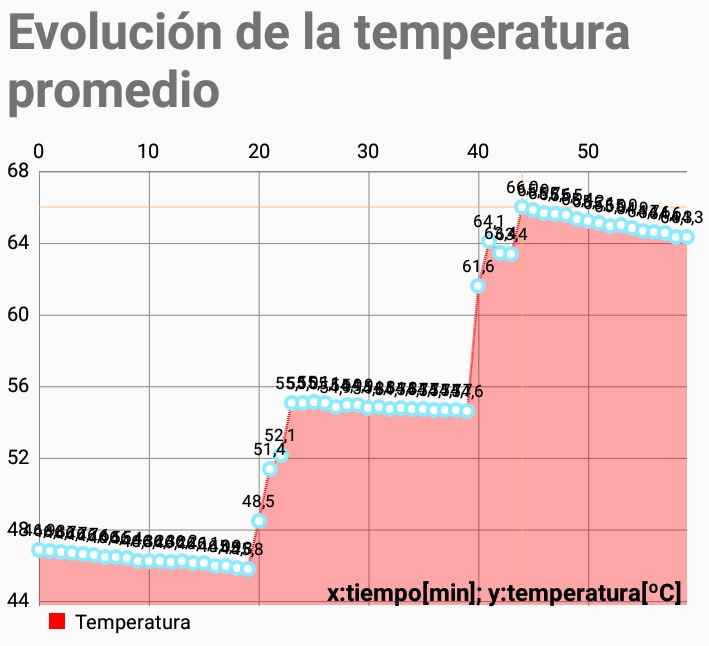
\includegraphics[scale=0.65]{Pruebas/EscalonadaEvolTempProm.jpg}
                \caption{Maceración escalonada: Evolución de la temperatura promedio de todos los Experimentos}
                \label{fig:EscTempProm}
            \end{figure}
        
            \begin{figure}[H]
                \centering
                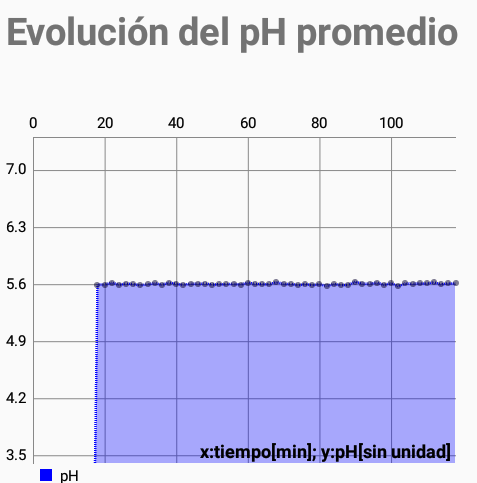
\includegraphics[scale=0.65]{Pruebas/EscalonadaEvolPhProm.jpg}
                \caption{Maceración escalonada: Evolución del pH promedio de todos los Experimentos}
                \label{fig:EscPhProm}
            \end{figure}     

\chapter{Metodologías ágiles de gestión}
\label{anexoMetodologiasAgiles}
\justifying
\par Las metodologías ágiles se basan en la utilización de una planificación poco exhaustiva y rígida en aras de facilitar la adaptación de las tareas según las necesidades que se presenten o los cambios en las prioridades que se requieran con la finalidad de cumplir los objetivos del proyecto.

\paragraph{Scrum:} Metodología de gestión ágil de proyectos, mayormente aplicada al software, basada en la  entrega de resultados con frecuencia constante (usualmente cada 2 o 4 semanas) y la integración del cliente en el proceso de desarrollo del proyecto.
% LIBRO INTRODUCCIÓN A SCRUM http://www.jeffsutherland.org/oopsla/schwapub.pdf

\paragraph{Kanban:} Metodología de gestión de actividades diseñada por Toyota\textsuperscript{®} y aplicada en software, basada en el control de un flujo secuencial de actividades. Uno de los principales conceptos aplicados es evitar el avance de ciertas actividades mientras no sea necesario o hasta que no se resuelvan conflictos o bloqueos que se presenten en el flujo de actividades. Al presentarse estas interrupciones, la práctica habitual es asignar mayor cantidad de recursos a la tarea bloqueada hasta que ésta se resuelva.